\documentclass[11pt,a4paper,twoside,openright]{report}

\usepackage{graphicx}
\usepackage{tabularx}
\usepackage{subfigure}
\usepackage{afterpage}
\usepackage{amsmath,amssymb}            
\usepackage{rotating}  
\usepackage{fancyhdr}  
\usepackage[scriptsize]{caption} 
\hyphenation{a-gen-tiz-za-zio-ne}

\setlength{\oddsidemargin}{2.cm}
\setlength{\evensidemargin}{2.cm}
\addtolength{\oddsidemargin}{-0.4cm}
\addtolength{\evensidemargin}{-0.4cm}
\linespread{1.1}

\usepackage[english]{babel}
\usepackage[latin1]{inputenc}
\renewcommand{\captionfont}{\normalfont \sffamily \itshape \small}

\pagestyle{empty}

\begin{document}
\thispagestyle{empty}
\vspace*{-1.5cm} \bfseries{
\begin{center}
	\LARGE
	POLITECNICO DI MILANO\\
	\vspace*{0.3cm}
	\normalsize
	School of Industrial and Information Engineering\\
	Master of Science in Computer Science and Engineering\\
	Dipartimento di Elettronica, Informazione e Bioingegneria\\
	\vspace*{0.8cm}
	\begin{figure}[htbp]
		\begin{center}
			
\includegraphics[width=5cm]{pictures/logo}
		\end{center}
	\end{figure}
	\vspace*{0.3cm} \LARGE
	\textbf{Assessing the Effectiveness of\\Rating Pattern Transfer Models\\for Recommender Systems}\\
	\vspace*{.75truecm} \large
\end{center}
\vspace*{2.0cm} \large
\begin{flushleft}
	Supervisor: Prof. Paolo Cremonesi\\
	Co-supervisor: Dott. Maurizio Ferrari Dacrema\\
\end{flushleft}
\vspace*{1.0cm}
\begin{flushright}
	Master's Thesis by:\\
	Giovanni Bozzano, 927867\\
\end{flushright}
\vspace*{1.0cm}
\begin{center}
	Academic Year 2020-2021
\end{center} \clearpage
}
\thispagestyle{empty} \normalfont \cleardoublepage
% \include{chapters/dedication}
% \thispagestyle{empty} \cleardoublepage
\pagenumbering{Roman}
\chapter*{Abstract}

With the ever increasing popularity of entertainment streaming services, social media, e-commerce websites etc., very large and diverse catalogs become usually hard to approach by users. Predicting the single customer's tastes and creating personalized lists of products has become a need for companies.\\
By aiming at alleviating this problem, recommender systems have recently become major players in the field of machine learning. These systems leverage the data of users and items of the catalog to extract information about each user's taste.\par
There are mainly two branches of recommender systems which differentiate by approach:
content-based recommender systems extract results based on item similarity, while collaborative filtering recommender systems take advantage of the user profiles and interactions history.\par
The quality of the results strictly depends on data quality and quantity. In particular, in practical applications, the amount of interactions has extremely low density compared to the whole dataset. That is, users tend to interact with or review a very small subset of the catalog. This issue is know as the data sparsity problem.\\
Over the years, many different knowledge transfer solutions to this problem have been proposed. The majority of these techniques relies on the overlap of users, items or both, between two dataset, source and target.\par
In this thesis we aim to analyse a particular set of knowledge transfer techniques based on rating pattern transfer, without any data overlapping between datasets. We show their formulation and performance with experiments on different datasets.
\thispagestyle{empty} \vspace*{.75truecm} \cleardoublepage
\chapter*{Acknowledgements}
\thispagestyle{empty} \vspace*{.75truecm} \normalfont \cleardoublepage
\pagestyle{plain}\renewcommand{\chaptermark}[1]{\markboth{\chaptername\ \thechapter.\ #1}{}} 
\renewcommand{\sectionmark}[1]{\markright{\thesection.\ #1}}         
\fancyhead[LE,RO]{\bfseries\thepage}    
                                        
\fancyhead[RE]{\bfseries\leftmark}    
\fancyhead[LO]{\bfseries\rightmark}     
\renewcommand{\headrulewidth}{0.3pt} 

\tableofcontents
\chapter{Introduction}

In recent years, due to the fast advancement of information technology, entertainment and commerce services have shifted towards the web medium.
Not only did consumers easily adapt to the new medium, but the expansion of options of what to do for fun has led to a major increase in entertainment activities related to digital media, which are now generally seen as an habit.\\
This, paired with continuously enriched and updated catalogs, makes sure that users are faced with a mass of media content. It is thus difficult for users to find the products they are interested in, while personal recommendations from friends or family is not enough to choose what to buy or how to employ free time. Recommender systems aim to address this issue and to increase traffic and revenue. There are two common types of recommender systems:
\begin{itemize}
\item Content-based: when catalog items are comparable, it is possible to leverage their features to retrieve items similar to the user's preferred ones. Generally, a similarity matrix is built by transforming the item features in numerical values and computing the distance between each interacted or liked item and the others.
\item Collaborative filtering: this technique aims at providing recommendations based on correlated preferences. Each user's historical interactions or preferences are used to determine the similarity with other users. Then, items preferred by similar users are recommended.
\end{itemize}
Both of these techniques suffer from poor data quality or quantity, which lead to wrong or biased user and item similarities.\\
Another common and major problem in the field of recommender systems is cold start.
The cold start problem arises when a user has no recorded interaction with any item or vice versa.\par
The objective of this thesis is to analyse a recent technique, called codebook transfer, which aims at alleviating these problems by transferring data from a different and unrelated dataset, with no overlap of users or items.\\
Since a set of articles expanding on the original technique have appeared over the last ten years, we evaluate the original codebook transfer model and a recent variation of it, called LKT-FM, by performing experiments targeting multiple domains and including different types of baselines.\par
By reporting multiple results, along with significance tests, and analysing the models, we show that the original technique, and thus the derived articles, only work on the specific scenarios reported in the original articles and that the base approach on which recent rating pattern transfer models are built is not capable of consistently transferring knowledge between non-overlapping domains.


\section{Thesis Structure}

The structure of the thesis is as follows.\\
\autoref{ch:state-of-the-art} describes the current state of the art in recommender systems. We present basic principles, classic and machine learning algorithms, evaluation criteria and knowledge transfer techniques.\\
\autoref{ch:analysed-models} contains a detailed description of the models of the analysed recommender systems that adopt the codebook transfer technique.\\
\autoref{ch:experiments-preprocessed} and \autoref{ch:experiments-full} include the description of datasets, parameters, goals and results of the experiments.\\
\autoref{ch:conclusion} contains the conclusion that can be drawn from the performed experiments and final notes.\\
\autoref{ch:applied-model} contains details about the implementations of the analysed recommender systems.\\
\autoref{ch:significance-tests} reports the tables of significance tests performed during the experiments.
\chapter{State of the Art}

In this chapter we describe the state of the art of recommender systems.\\
In the first section we start from the basic principles of recommender systems, covering the standard techniques, such as content-based, collaborative and hybrid recommender systems. After that, we will cover the matrix factorization model.\\
In the second section we will cover the metrics used to evaluate datasets and recommender systems results.\\
The third sections describes the state of the art of knowledge transfer techniques used in recommender systems.\\
The fourth section describes clustering techniques and their use in recommender systems.



\section{Basic principles of Recommender Systems}

In this section we will start by giving a brief definition of recommender systems and the problems they are faced with.\\
The most accurate definition of modern recommender systems can be found in Burke's statement:\\
"Any system that produces individualized recommendations as output or has the effect of guiding the user in a personalized way to interesting or useful objects in a large space of possible options." (Burke, 2002)


\subsection{Recommender Systems Tasks}

While recommender systems in general are aiming at learning and anticipate user preferences to provide helpful suggestions, they are faced with two distinct tasks: items ranking and items ratings prediction.\\
Ranking is the task of selecting from the whole catalog a small number of items to be recommended for each user. We can distinguish two slightly different scenarios for the ranking task. If an item of the catalog can be interacted with multiple times, every item should be eligible for recommendation. For example, in a music streaming service, users usually listen to the same song several times. On the contrary, if users are not expected to choose the same item twice, already rated or seen items are excluded from the items the recommender systems suggests.\\
Rating prediction consists in providing a computed rating for each user unrated item. Since items with predicted ratings can then be ordered and selected for ranking, most of the times the two tasks share some characteristics, while the main differences between them are identified in the evaluation test set and metrics.


\subsection{Types of Feedback}

Since recommender systems can leverage historical data and user profiles, it is important to distinguish two types of feedback.
Explicit feedback are clear and numerical values of how much a user liked or disliked an item he interacted with.
While explicit feedback is the most accurate indicator of user preferences and, for this reason, it makes the recommendation task easier, they are usually hard to obtain from users, since a user input is required. Additionally, explicit feedback can easily be user biased, as different users could value a numeric rating differently.\\
Implicit feedback is identified as the user interaction with an item. For example, the action of listening to a song on a streaming service is considered implicit feedback.
Implicit feedback cannot differentiate between positive and negative feedback and as such it is always available but considered less reliable than explicit ratings.


\subsection{Data Structures}

Recommender systems often make use of common data structures, which can identified in the following matrices:

\begin{itemize}

\item \textbf{User-Content Matrix (UCM)}: Given a set of users $U$ and a set of user labels $L$, the UCM is a matrix with shape $|U| \times |L|$ where each row represents a user $u \in U$ and each column represents a label $l \in L$. Each cell $(u,l)$ represents the value of label $l$ of the user $u$. It can be a real, integer or binary value depending on the nature of the label. For example, to describe the user age, we could either have a single integer label, where each cell value would represent the age of the user, or multiple binary labels representing different age brackets, where each cell value would be:
\begin{equation}
  (u,l)=
  \begin{cases}
    0, & \text{if}\ u\ \text{belongs to the age bracket}\ l\\
    1, & \text{otherwise}
  \end{cases}
\end{equation}
The approach of splitting a numerical label into multiple categorical labels is called one-hot encoding.\\
The UCM is generally built in content based recommendation approaches.

\item \textbf{Item-Content Matrix (ICM)}: Given a set of items $I$ and a set of item labels $L$, the ICM is a matrix with shape $|I| \times |L|$ where each row represents an item $i \in I$ and each column represents a label $l \in L$. Each cell $(i,l)$ represents the value of label $l$ of the item $i$. It can be a real, integer or binary value depending on the nature of the label.\\
Similarly to the UCM, the ICM is generally built in content based recommendation approaches.

\item \textbf{Similarity Matrix}: Given a set of items $I$, the similarity matrix is a matrix with shape $|I| \times |I|$ where each row $i_r$ and column $i_c$ represent an item $i \in I$ and each cell represent the similarity between $i_r$ and $i_c$. The same structure is used for user similarity.

\item \textbf{User-Rating Matrix (URM)}: Given a set of users $U$ and a set of items $I$, the URM is a matrix with shape $|U| \times |I|$ where each row represents a user $i \in I$ and each column represents an item $i \in I$. Each cell $(u,i)$ represents the value of the rating of the item $i$ by user $u$. It can be a real, integer or binary value depending on the nature of the feedback. For example, in the scenario of explicit feedback, each cell would have a real or integer value, usually with upper and lower bounds, while in the scenario of an implicit feedback, each cell value would be:\\
\begin{equation}
  (u,l)=
  \begin{cases}
    0, & \text{if}\ u\ \text{interacted with item}\ i\\
    1, & \text{otherwise}
  \end{cases}
\end{equation}
The URM is generally built in collaborative filtering recommendation approaches.

\end{itemize}


\subsection{Similarities}

A similarity function is mathematical tool to compute the similarity between two entities represented in a space, as a numerical value. In the field of recommender systems similarity functions are often used to extract similar entities from a dataset, given a target user or item. It is then important to mention and describe the commonly used ones.

\begin{itemize}

\item \textbf{Cosine similarity}: given two vectors $x$ and $y$, the cosine similarity is computed as follows:
\[ S_{xy} = \frac{x \times y}{||x||\||y|| + h} \]
where $h$ is the shrink term for normalization.
This similarity measures the angle between n-dimensional vectors. Since the angle can vary between 1 and -1, $S_{xy} \in [-1, 1]$. If $S_{xy} = 1$ we have complete similarity (parallel vectors); if $S_{xy} = 0$, we have no similarity (orthogonal vectors) and if $S_{xy} = -1$ we have inverse similarity (parallel vectors with inverse direction).\\
The cosine similarity is between the two most popular similarities used in recommender systems.

\item \textbf{Pearson correlation}: given two random variables $X$ and $Y$, the Pearson correlation can be computed as follows:
\[ \rho_{X,Y} = \frac{cov(X,Y)}{\sigma_x \sigma_y} \]
where $cov(X,Y)$ is the covariance between $X$ and $Y$ and $\sigma_x$ and $\sigma_y$ are respectively the standard deviations of $X$ and $Y$.\\
Since we need to apply the formula to a sample, we can give the following definition. Given two vectors $x$ and $y$ of dimension $n$, the pearson correlation is computed as follows:
\[ S_{xy} = \frac{\sum_{i}^{n} (x_i - \bar{x})(y_i - \bar{y})}{\sqrt{\sum_{i}^{n} (x_i - \bar{x})^2}\sqrt{\sum_{i}^{n} (y_i - \bar{y})^2} + h} \]
where $\bar{x}$ and $\bar{y}$ are respectively the means of $x$ and $y$ and $h$ is the shrink term for normalization.\\
Like with the cosine similarity $S_{xy} \in [-1, 1]$, where -1 means positive linear correlation, 0 means no linear correlation and -1 means negative linear correlation. It is very popular in recommender systems.

\item \textbf{Jaccard coefficient}: given two vectors $x$ and $y$, the Jaccard coefficient is computed as follows:
\[ S_{xy} = \frac{x \times y}{|x| + |y| - xy + h} \]
where $h$ is the shrink term for normalization.\\
The Jaccard coefficient is ranged in the interval $[0, 1]$ and is used to compute the similarity between two finite sets and can be applied with binary values.

\item \textbf{Dice coefficient}: given two vectors $x$ and $y$, the Dice coefficient is computed as follows:
\[ S_{xy} = \frac{x \times y}{\frac{1}{2}|x| + \frac{1}{2}|y| - xy + h} \]
where $h$ is the shrink term for normalization.\\
It ranges in the interval $[0, 1]$ and, like the Jaccard coefficient, it is used to compute the similarity between finite sets and can be applied with binary values.

\item \textbf{Tanimoto coefficient}: given two vectors $x$ and $y$ of dimension $n$, the Tanimoto coefficient is computed as follows:
\[ S_{xy} = \frac{\sum_{i = 1}^{n} x_iy_i}{\sum_{i = 1}^{n} x_i^2 + \sum_{i = 1}^{n} y_i^2 - \sum_{i = 1}^{n} x_iy_i} \]
where $h$ is the shrink term for normalization.\\
It ranges in the interval $[0, 1]$ and, like Jaccard and Dice coefficients, it is used to compute the similarity between finite sets and can be applied with binary values.

\end{itemize}



\section{Types of Recommender Systems}

There exist several types of recommender systems, but they can mainly be divided into three macro-types.


\subsection{Content-based Filtering (CBF)}

When users or items characteristics are available, it is possible to leverage them to create personalized recommendations. For example, clothing digital stores may use colors of clothing as a label to compute items similarity. The objective of this type of recommender systems is to use one or more labels for each user or item, starting from their characteristics, and exploit them to identify similar entities. We can distinguish between item-based and user-based CBF.

\begin{itemize}

\item \textbf{Item-based}: given the set of items $I$ and the set of users $U$, for each user $u \in U$ we define $I_u$ as the set of items rated by user $u$. To recommend items to user $u$, the system exploits the ICM to compute the similarities between each item $i_u \in I_u$ and $i \in I$ by building an item similarity matrix with shape $|I_u| \times |I|$.\\
Then, it computes the estimated rating of each item $i$ by user $u$ as follows:
\[ \hat{r}_{ui} = \frac{\sum_{i_u \in I_u} r_{ui_u} * ISIM_{i_u,i}}{\sum_{i_u \in I_u} ISIM_{i_u,i}} \]
where $r_{ui_u}$ is the rating of item $i_u$ by user $u$ and $ISIM$ is the item similarity matrix. The normalization is useful to compute accurate ratings, but can be left out for top-n recommendation.\\
Items with the highest ratings, excluding items in $I_u$, are recommended to user $u$.
To avoid computing the similarity matrix for each user, it is possible to build a single item similarity matrix with shape $|I| \times |I|$ and consider, for each user, only the items contained in $I_u$.

\item \textbf{User-based}: given the set of items $I$ and the set of users $U$, for each user $u \in U$ we define $I_u$ as the set of items rated by user $u$. Similarly to the item-based approach, a user similarity matrix with shape $|U| \times |U|$ is built starting from the UCM.\\
The estimated rating of each item $i \in I$ by user $u$ is computed as follows:
\[ \hat{r}_{ui} = \frac{\sum_{v \in U} r_{vi_u} * USIM_{u,v}}{\sum_{v \in U} USIM_{u,v}} \]
Items with the highest ratings, excluding items in $I_u$, are recommended to user $u$.

\end{itemize}

The main advantage of CBF is that it makes possible to solve the cold start problem, both for users and items, when their features are available. By leveraging the users and items features to provide recommendations, CBF bypasses the problem completely.


\subsection{Memory-based Collaborative Filtering}

Memory-based collaborative filtering recommender systems exploit the assumption that similar users will likely prefer the same items. They use interactions as a bridge to identify similar users or items, called neighbors. The goal of this approach is then to compute a neighborhood for target users or items. In order to describe the methodology, we must distinguish between user-based and item-based.

\begin{itemize}

\item \textbf{User-based}: in the user-based approach, the goal of the system is to compute a neighborhood for the user $u$ needing recommendations. This is defined as the set of users similar to $u$ based on their preferences. Their own preferences are then used to extract recommendation for the user $u$.\\
Given the set of users $U$ and the set of items $I$, the system exploits the URM to build a user similarity matrix with shape $|U| \times |U|$.\\
We define $URM_u$ as the set of items rated by user $u$ and $URM_{u,i}$ as the rating of item $i$ by user $u$.\\
The estimated rating of each item $i \in I$ by user $u$ is computed as follows:
\[ \hat{r}_{ui} = \frac{\sum_{v \in U \wedge v \neq u} URM_{v,i} * USIM_{u,v}}{\sum_{v \in U} USIM_{u,v}} \]
Items with the highest ratings, excluding items in $URM_u$, are recommended to user $u$.

\item \textbf{Item-based}: the item-based approach is slightly different. In this scenario, the system computes the neighborhood of the item $i$ and then recommends it to users belonging to the neighborhood that are yet to interact with it.\\
Given the set of users $U$ and the set of items $I$, the system exploits the URM to build an item similarity matrix with shape $|I| \times |I|$.\\
Like in the user-based approach, we define $URM_u$ as the set of items rated by user $u$ and $URM_{u,i}$ as the rating of item $i$ by user $u$.\\
The estimated rating of each item $i \in I$ by user $u$ is computed as follows:
\[ \hat{r}_{ui} = \frac{\sum_{j \in I \wedge j \neq i} URM_{u,j} * USIM_{i,j}}{\sum_{j \in I} USIM_{i,j}} \]
Items with the highest ratings, excluding items in $URM_u$, are recommended to user $u$.

\end{itemize}


\subsection{Model-based Collaborative Filtering}

Model-based collaborative filtering recommender systems exploit the URM with a machine learning model to provide recommendations. There are many different ways to do so and in this thesis we will cover matrix factorization in \autoref{matrix-factorization} and factorization machines in \autoref{factorization-machines}.


\subsection{Hybrid}

Different recommender systems have different strengths and weaknesses. Many different types of hybrid systems have been developed to overcome the weaknesses of the single approaches. There are multiple techniques that can be used to combine the results. The most common technique is to combine the items scores into a single recommendations by assigning weights. Alternatives are switching recommender system based on the scenario or to use different systems in cascade to refine previous recommendations.



\section{Matrix Factorization}
\label{matrix-factorization}

Matrix factorization \cite{10.1109/MC.2009.263} is a way of computing matrix decomposition: reducing a matrix into the product of two other matrices. After winning the Netflix Prize competition in 2009, it became a very popular approach in recommender systems.\par
The assumption of matrix factorization is that it is possible to extract latent factors, to characterize users and items, from the rating pattern. For items, these factors represent an alternative to the human generated features. For users, the factors represent how much a user prefers items with a high score in the corresponding factor. For this reason, we say that matrix factorization is an approach for latent factors models.\par
Given a set of users $U$ and a set of items $I$, matrix factorization models decompose the URM so that users and items are mapped to a latent factor space of dimensionality $f$ and their interactions are modeled as inner products in that space. Each user $u \in U$ is associated with a vector $p_u \in \mathbb{R}^f$ and each item $i \in I$ is associated with a vector $q_i \in \mathbb{R}^f$.\\
For each user $u$, the values of $p_u$ measure how much the user likes items characterized by the corresponding factor. For each item $i$, the values of $q_i$ measure how much the item is characterized by that factor.\\
The estimated rating of item $i$ by user $u$ is then computed as follows:
\[ \hat{r}_{ui} = q_i^T p_u \]\\
The challenge of matrix factorization is building the mappings for users and items.


\subsection{Stochastic Gradient Descent (SGD)}

SGD is a popular approach \cite{ImprovingSVD, 10.1145/1401890.1401944, 10.1145/1345448.1345466} to compute the latent factors mappings. It involves cycling all the training ratings and computing the error:
\[ e_{ui} = r_{ui} - q_i^T p_u \]
Then, the values are modified by a magnitude proportional to $\gamma$ in the opposite direction of the gradient, as follows:
\begin{equation*}
\begin{split}
& p_u \gets p_u + \gamma (e_{ui} q_i - \lambda p_u) \\
& q_i \gets q_i + \gamma (e_{ui} p_u - \lambda q_i)
\end{split}
\end{equation*}
where the costant $\lambda$ determines the extent of regularization.



\section{Factorization Machines (FM)}
\label{factorization-machines}

Factorization machines \cite{10.1109/ICDM.2010.127} are a relatively new technique of collaborative filtering with side information proposed by Steffen Rendle in 2010. Since they are a general-purpose supervised learning algorithm, they can be adapted to work with recommender systems.\\
Given $S$ the set of tuples $(\bar{x}, y)$ where $\bar{x} = (x_1, ..., x_k) \in \mathbb{R}^k$ is a k-dimensional feature vector and $y$ is the corresponding class label, using factorized interactions, FM models all possible interactions between variables in $\bar{x}$.\\
The FM model equation is defined as follows:
\begin{equation*}
\hat{y}(\bar{x}) = w_0 + \sum_{i = 1}^{n} w_i x_i + \sum_{i = 1}^{n} \sum_{j = i + 1}^{n} \langle v_i, v_j \rangle x_i x_j
\end{equation*}
where $w_0 \in \mathbb{R}$ is the global bias, $w_i \in \mathbb{R}$ is the bias of feature $i$, vector $v_i \in \mathbb{R} \times f$ is the interaction parameter vector of feature $i$ and $\langle \cdot, \cdot \rangle$ is the dot product of two vectors of size k:
\begin{equation*}
\langle v_i, v_j \rangle = \sum_{f = 1}^{k} v_{i,f} \cdot v_{j,f}
\end{equation*}



\section{Dataset Metrics}

The main characteristic of a dataset is sparsity. Given a user rating matrix, sparsity is the ratio of observed to total ratings. %(https://arxiv.org/pdf/1205.3193.pdf)



\section{Data Partitioning}

To address the evaluation of a recommender system, it is important to introduce in detail the different methodologies of how it can be performed.\\
There can be three types of evaluation:

\begin{itemize}
\item \textbf{Online evaluation}: a controlled environment is set up and a group of selected users is asked to use it and to report on the experience.
\item \textbf{Live trials}: similarly to the previous methodology, it is performed by real users. With this approach, real users are asked to provide feedback in a production environment.
\item \textbf{Offline evaluation}: the most used evaluation technique consists in analyzing past user interactions. Since in offline evaluation no new rating is given after the model is trained, it is necessary to simulate a test set of ratings by splitting the original dataset into multiple subsets. Hence, the need to introduce the different approaches to data partitioning.
\end{itemize}

Data partitioning for offline evaluation is generally performed for cross-validation. Cross-validation is the approach of splitting the original dataset into three subsets:
\begin{itemize}
\item \textbf{Training set}: this set is used to train the model. Normally, to maximize the training efficiency, it is the biggest of the three sets.
\item \textbf{Validation set}: this set is used to evaluate the model during training and optimize the model hyperparameters.
\item \textbf{Test set}: this set is used to perform the final evaluation, after the training is finished, to test the recommender system performance with data it has never seen before.
\end{itemize}
While the validation and test sets could technically overlap, this would lead to overfitting. Overfitting is an error that occurs when a model is very efficient in providing recommendations for a restricted set of data but is unable to generalize to new scenarios.

There exist many different techniques to build the three subsets. We will cover the most widely used:

\begin{itemize}
\item \textbf{Holdout}: it is the simplest approach to data partitioning. After specifying a size to each subset, each user-item interaction is assigned to one of the three subsets randomly or following \textit{leave-k-out} logic.\\
With leave-k-out, for each user, $k$ interactions are assigned to the validation set and $k$ interactions are assigned to the test set.
\item \textbf{K-Fold}: it splits the original in $k$ \textit{folds}. Each fold is then used in turn as train, validation or test set. For this reason, the amount of iterations to evaluate the model is equal to the amount of folds.\\
With K-Fold the recommender system is evaluated with multiple data partition samples, thus allowing a better estimation of the model performance.
\end{itemize}



\section{Evaluation Metrics}

When designing or evaluating a recommender system, metrics a fundamental point to understand and use correctly. Depending on the characteristics that need to be evaluated, different sets of metrics have different meanings.


\subsection{Accuracy metrics}

Accuracy metrics are meant to evaluate ranking. They measure the predictiveness of the recommender system; how good its decisions are. The most popular accuracy metrics are Mean Average Precision (mAP) and Normalized Discounted Cumulative Gain (nDCG). Both of them evaluate how good the recommender is to put the most relevant items first in the recommendation list.\par
mAP is outfitted with a top-n threshold which defines how many recommended items are considered for the metric computation. mAP@n is then used to indicate mAP computed on the first n items recommended to each user.\\
We define Precision of the query for user $i$ as
\[ P@k_i = \frac{relevant\_items@k_i}{k} \]
Where $relevant\_items@k$ is the amount of relevant items included in the recommendations list up to rank $k$.\\
We then define Average Precision of the query for user $i$ as
\[ AP@n_i = \frac{1}{TP} \sum_{k=1}^{n} (P@k_i * rel@k) \]
where $TP$ is the total amount of ground truth items and $rel@k$ equals 1 if the item at rank k is relevant and equals to 0 otherwise.\\
Finally, mAP is defined as
\[ mAP@n = \frac{1}{U} \sum_{i=1}^{U} AP@n_i \]
where $U$ is the amount of users.\par
Like mAP, nDCG is computed with a top-n threshold.\\
We define Cumulative Gain as
\[ CG@n = \sum_{k=1}^{n} rating@k \]
where $rating@k$ is the predicted rating of the item at rank $k$.\\
Discounted Cumulative Gain is then computed to penalize ratings based on their position
\[ DCG@n = \sum_{k=1}^{n} \frac{rating@k}{\log(i+1)} \]
Then the result is normalized to make it irrelevant of the query. To do so, we compute the Ideal DCG
\[ IDCG@n = \sum_{k=1}^{|REL_n|} \frac{rating@k}{\log(i+1)} \]
where $REL_p$ is the list of relevant items up to position $n$.\\
Finally, nDCG is defined as
\[ nDCG@n = \frac{DCG@n}{IDCG@n} \]


\subsection{Error metrics}

Error metrics are used to compare actual and predicted ratings, thus are generally used for rating prediction. The most commonly used error metrics are Mean Absolute Error (MAE) and Root Mean Squared Error (RMSE).
MAE is defined as
\[ MAE = \frac{1}{U*I} \sum_{u=1}^{U} \sum_{i=1}^{I} |r_{u,i} - \hat{r}_{u,i}| \]
where $U$ is the amount of users, $I$ is the amount of items, $r_{u,i}$ is the predicted rating of item $i$ by user $u$ and $r_{u,i}$ is the true rating of item $i$ by user $u$.\\
As the formula suggests, MAE does not apply a different weight to outliers, large error values.\\
To compute a weighted error, we define RMSE as
\[ RMSE = \sqrt{\frac{1}{U*I} \sum_{u=1}^{U} \sum_{i=1}^{I} (r_{u,i} - \hat{r}_{u,i})^2} \]


\subsection{Diversity}

Gini index, or Gini coefficient, is a well known statistical metric used to measure income inequality. It can be slightly changed in and used in the field of recommender systems to evaluate a system diversity. We call the variation, where higher values mean higher diversity, Gini diversity \cite{Diversity}.\\
It is computed as follows:
\[ gini\_diversity = 2 \sum_{i=1}^{n} \frac{(n + 1 - i) * x_i}{(n + 1) * \sum_{i=1}^{n} x_i} \]
where $n$ is the amount of items and $x_i$ is the numbers of times item $i$ has been recommended.



\section{Clustering Techniques}

Clustering is the operation of grouping similar unclassified elements together according to some properties or features. It is used in many fields of machine learning with different applications and implementations. In this section we cover the main clustering algorithms used in recommender systems, paying particular attention to the one used in this thesis.


\subsection{K-Means Clustering}

K-Means clustering is the most used and well-known iterative clustering algorithm.\\
To apply K-Means clustering it is necessary to define the number of target clusters. For each cluster, a centroid with random coordinates is initialized.
\begin{itemize}
\item Each element is classified by computing the euclidean distance between its position in space and each centroid. The element is assigned to closest centroid.
\item The centroid is moved by computing the mean of the distances between it and all the elements assigned to it.
\item The process is repeated until the the centroid are only slightly moved or until a maximum amount of iterations is reached.
\end{itemize}
\begin{figure}[htbp]
	\begin{center}
		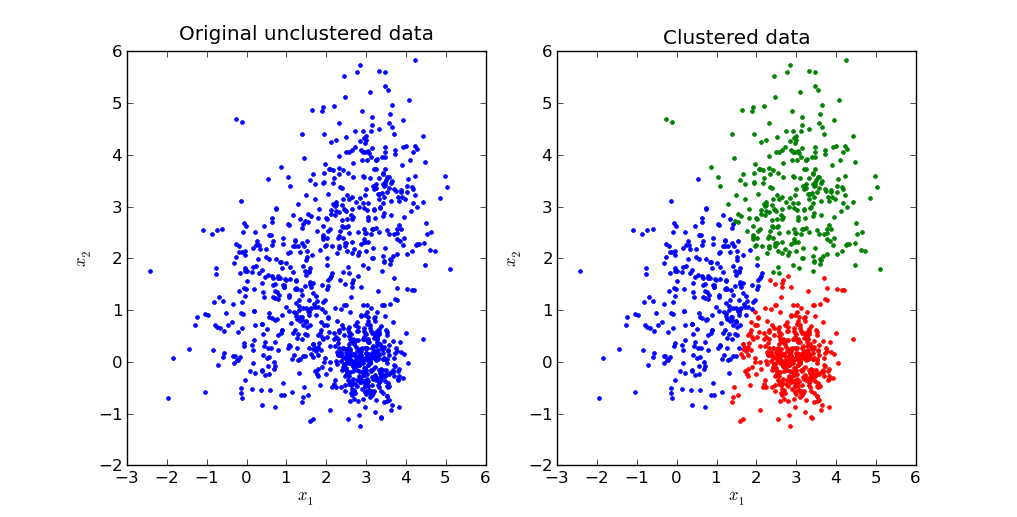
\includegraphics[width=\textwidth]{pictures/k-means-clustering}
		\caption{Results of the K-Means clustering algorithm. Source: https://i.stack.imgur.com/cIDB3.png}
	\end{center}
\end{figure}
K-Means clustering has linear complexity $O(n)$, thus it is considered a fast clustering algorithm.


\subsection{Non-Negative Matrix Factorization (NMF)}

Non-Negative matrix factorization is a set of algorithms for high dimensional data analysis that extracts features from a set of non-negative vectors. It was first introduced by an article by Paatero and Tapper in 1994 \cite{10.1002/env.3170050203} and has been widely used ever since it was made popular by Lee and Seung in 1999 \cite{10.1038/44565}, with the first simple algorithm.\\
It has been proved empirically by different experiments \cite{10.5555/1005332.1044709, 10.1109/CVPR.2001.990477} that NMF has clustering effects.
Given a metrix $X$ with shape $m \times n$, the goal of NMF is to compute matrices $F$, with shape $m \times p$, and $G$, with shape $p \times n$, such that:
\begin{equation*}
X = FG
\end{equation*}
by solving the optimization problem:
\begin{equation*}
\min_{F \in \mathbb{R}^{m \times p}_+, G \in \mathbb{R}^{p \times n}_+} ||X - FG||^2_F
\end{equation*}
where $||X - FG||^2_F$ is the Frobenius norm, defined as:
\begin{equation*}
||X - FG||^2_F = \sum_{i,j} (X - FG)^2_{i,j}
\end{equation*}
The standard NMF algorithm is the following:
\vskip 0.7cm
\begin{algorithm}[H]
\SetKwInOut{Input}{Input}
\SetKwInOut{Output}{Output}
\Input{Non-negative matrix $X \in \mathbb{R}^{m \times n}_+$ and factorization rank $r$.}
\Output{$(F,G) \geq 0$ : A rank-$r$ NMF of $X \approx FG$.}
Generate initial matrices $F^{(0)} \geq 0$, $G^{(0)} \geq 0$\;
\For{$t \gets 1$ \KwTo $max\_iteration$}{
  $G^{(t)} \gets G^{(t - 1)} \odot \frac{(F^{(t - 1)})^T X}{(F^{(t - 1)})^T F^{(t - 1)} G^{(t - 1)}}$\;
  $F^{(t)} \gets F^{(t - 1)} \odot \frac{X (G^{(t)})^T}{F^{(t - 1)} G^{(t)} (G^{(t)})^T}$\;
}
\caption{The standard algorithm for NMF}
\end{algorithm}
\vskip 0.7cm
$F$ and $G$ can be initialized randomly or using some other clustering method, such as K-Means clustering.


\subsection{Orthogonal Non-Negative Matrix Tri-Factorizations (ONMTF)}

Orthogonal non-negative matrix factorizations (ONMF) is a type of NMF that, given a matrix $X$ with shape $m \times n$, computes matrices $F$, with shape $m \times p$, and $G$, with shape $n \times p$, such that:
\begin{equation*}
X = FG^T
\end{equation*}
by solving the optimization problem:
\begin{equation*}
\min_{F \in \mathbb{R}^{m \times p}_+, G \in \mathbb{R}^{p \times n}_+} ||X - FG^T||^2_F, \quad \text{s.t.} \quad F^TF = I
\end{equation*}
Alternatively, for the $G$-orthogonal problem is:
\begin{equation*}
\min_{F \in \mathbb{R}^{m \times p}_+, G \in \mathbb{R}^{p \times n}_+} ||X - FG^T||^2_F, \quad \text{s.t.} \quad G^TG = I
\end{equation*}
The algorithms for ONMF are the following:
\vskip 0.7cm
\begin{algorithm}[H]
\SetKwInOut{Input}{Input}
\SetKwInOut{Output}{Output}
\Input{Non-negative matrix $X \in \mathbb{R}^{m \times n}_+$ and factorization rank $r$.}
\Output{$(F,G) \geq 0$ : A rank-$r$ NMF of $X \approx FG^T$.}
Generate initial matrices $F^{(0)} \geq 0$, $G^{(0)} \geq 0$\;
\For{$t \gets 1$ \KwTo $max\_iteration$}{
  $G^{(t)} \gets G^{(t - 1)} \odot \frac{X^T F^{(t - 1)}}{G^{(t - 1)} (F^{(t - 1)})^T F^{(t - 1)}}$\;
  $F^{(t)} \gets F^{(t - 1)} \odot \sqrt{\frac{X G^{(t)}}{F^{(t - 1)} (F^{(t - 1)})^T X G^{(t)}}}$\;
}
\caption{The algorithm for $F$-orthogonal ONMF}
\end{algorithm}
\vskip 0.7cm
\begin{algorithm}[H]
\SetKwInOut{Input}{Input}
\SetKwInOut{Output}{Output}
\Input{Non-negative matrix $X \in \mathbb{R}^{m \times n}_+$ and factorization rank $r$.}
\Output{$(F,G) \geq 0$ : A rank-$r$ NMF of $X \approx FG^T$.}
Generate initial matrices $F^{(0)} \geq 0$, $G^{(0)} \geq 0$\;
\For{$t \gets 1$ \KwTo $max\_iteration$}{
  $G^{(t)} \gets G^{(t - 1)} \odot \sqrt{\frac{X^T F^{(t - 1)}}{G^{(t - 1)} (G^{(t - 1)})^T X^T F^{(t - 1)}}}$\;
  $F^{(t)} \gets F^{(t - 1)} \odot \frac{X (G^{(t)})^T}{F^{(t - 1)} (G^{(t)})^T G^{(t)}}$\;
}
\caption{The algorithm for $G$-orthogonal ONMF}
\end{algorithm}
\vskip 0.7cm
The tri-factorizations \cite{10.1145/1150402.1150420} variant uses three factors instead of two, in the form:
\begin{equation*}
X = FSG^T
\end{equation*}
The optimization problem is the following:
\begin{equation*}
\min_{F \in \mathbb{R}^{m \times p}_+, G \in \mathbb{R}^{p \times n}_+, S \in \mathbb{R}^{p \times r}_+} ||X - F S G^T||^2_F, \quad \text{s.t.} \quad F^TF = I, G^TG = I
\end{equation*}
According to Ding \textit{et al} \cite{10.1145/1150402.1150420}, tri-factorization is capable of clustering rows and columns of the input matrix simultaneously.\\
The rules for updating $F$, $G$ and $S$, are according to the following algorithm:
\vskip 0.7cm
\begin{algorithm}[H]
\SetKwInOut{Input}{Input}
\SetKwInOut{Output}{Output}
\Input{Non-negative matrix $X \in \mathbb{R}^{m \times n}_+$ and factorization rank $r$.}
\Output{$(F,G,S) \geq 0$ : A rank-$r$ NMF of $X \approx FSG^T$.}
Generate initial matrices $F^{(0)} \geq 0$, $G^{(0)} \geq 0$, $S^{(0)} \geq 0$\;
\For{$t \gets 1$ \KwTo $max\_iteration$}{
  $G^{(t)} \gets G^{(t - 1)} \odot \sqrt{\frac{X^T F^{(t - 1)} S^{(t - 1)}}{G^{(t - 1)} (G^{(t - 1)})^T X^T F^{(t - 1)} S^{(t - 1)}}}$\;
  $F^{(t)} \gets F^{(t - 1)} \odot \sqrt{\frac{X G^{(t)} (S^{(t - 1)})^T}{F^{(t - 1)} (F^{(t - 1)})^T X G^{(t)} (S^{(t - 1)})^T}}$\;
  $S^{(t)} \gets F^{(t - 1)} \odot \sqrt{\frac{(F^{(t)})^T X G^{(t)}}{(F^{(t)})^T F^{(t)} S^{(t - 1)} (G^{(t)})^T G^{(t)}}}$\;
}
\caption{The algorithm for ONMTF}
\end{algorithm}



\section{Cross-Domain Recommender Systems}

While the majority of recommender systems provide recommendation targeted only to a single topic, in recent years large digital service companies like Amazon or Google started providing recommendation across a very eterogeneous set of services. Amazon, for example, provides recommendations both for its e-commerce website, for items of all categories, and for music, movies and so on. In this scenario it may be useful to provide recommendation across different domains.\par
Cross-domain recommender systems aim to generate higher quality recommendations in a target domain by leveraging data coming from one more different source domains. In particular, knowledge acquired in a source domain can be transferred with some knowledge-transfer technique to the target domain.\\
The use cases for such approach are mainly two. First, building a user profile across domains allows to generate bundle recommendation \cite{10.1007/s11257-012-9131-2, 10.1007/s11257-007-9042-9, 10.1007/s11257-012-9128-x}. For example it may be possible to recommend the movie transposition of a book the user bought and then to recommend the movie soundtrack. A recommendation like that can only be inferred by exploiting data from multiple domains. The second scenario is the one of the cold start problem \cite{10.1145/2645710.2645777, 10.1007/978-3-642-22362-4_26, 10.1145/2507157.2507206}. Auxiliary source domain may be able information which is missing in the target domain. Both of these scenarios assume that there are correspondences between user and item profiles across domains.\par
A complete review of recommender systems was given by Cremonesi \textit{et al} \cite{10.1007/978-1-4899-7637-6_27}. To introduce their properties and categories we mainly follow their formalization of the problem.


\subsection{Domain Definitions}

The first step in introducting cross-domain recommender systems, is defining the concept of domain. We can distinguish four different levels of domain definition:
\begin{itemize}
\item \textbf{Attribute level}: Two items are considered to belong to different domains if they differ in some attribute. For example two books could be considered of different domains if the differ by genre. The attribute level definition is too weak to be considered for cross-domain recommender systems.
\item \textbf{Type level}: Two items are considered to belong to different domains if they share some attributes but differ by others. For example, TV series and movies belong to different domains, according to this definition.
\item \textbf{Item level}: Two items are considered to belong to different domains if they don't share any attribute, or at least very few. For example, movies and books belong to different domains, according to this definition.
\item \textbf{System level}: Two items are considered to belong to different domains if they belong to different systems, even if they share the same attributes. For example, movies from the Netflix system and movies from the Amazon system belong to different domains, according to this definition.
\end{itemize}


\subsection{Types of recommendation}

The goal of cross-domain recommender systems can also vary depending on which domain is the target for recommendations.\\
According to Cremonesi \textit{et al} \cite{10.1007/978-1-4899-7637-6_27}, we can distinguish three types of recommendations. Given the target domain $D_T$ with its users and items sets, respectively $U_T$ and $I_T$, and one or more source domains $D_S$ with their users and items sets, respectively $U_S$ and $I_S$, we distinguish the following types or recommendation types:
\begin{itemize}
\item \textbf{Multi-domain recommendation}: recommend items in $I_S \cup I_T$ to users in $U_S$ or to users in $U_T$. This approach requires a significant amount of users overlap between domains, but it is becoming feasible due to the amount of profiles maintained by users on different social media, connected by mechanisms of cross-authentication and identification \cite{10.1016/j.ins.2008.08.022} or interoperability \cite{10.1007/s11257-011-9097-5}.
\item \textbf{Linked-domain recommendation}: recommend items in $I_T$ to users in $U_S$ or $U_T$ by exploiting knowledge about $U_S \cup U_T$ and $I_S \cup I_T$. This approach is used to enrich data in a target domain with a cold start or data sparsity problem. Generally, it requires at least a partial amount of users or items overlap between the source and target domains.
\item \textbf{Cross-domain recommendation}: recommend items in $I_T$ to users in $U_S$ or $U_T$ by exploiting knowledge about $U_S$ and $I_S$. This approach is used when the target domain has no information about the users. In this scenario there is no assumption of data overlap between domains and the approaches aim at transferring knowledge from one domain to the other.
\end{itemize}


\subsection{Types of Overlap}

We can then make distinction between four types of overlap:
\begin{itemize}
\item \textbf{No overlap}: Neither the user nor the item sets share common data, such that:
\begin{equation*}
U_T \cap U_S = \emptyset \quad \text{and} \quad I_T \cap I_S = \emptyset
\end{equation*}
\item \textbf{User overlap}: Only the user sets share common data, such that:
\begin{equation*}
U_T \cap U_S \neq \emptyset \quad \text{and} \quad I_T \cap I_S = \emptyset
\end{equation*}
\item \textbf{Item overlap}: Only the item sets share common data, such that:
\begin{equation*}
U_T \cap U_S = \emptyset \quad \text{and} \quad I_T \cap I_S \neq \emptyset
\end{equation*}
\item \textbf{User and item overlap}: Both user and item sets share common data, such that:
\begin{equation*}
U_T \cap U_S \neq \emptyset \quad \text{and} \quad I_T \cap I_S \neq \emptyset
\end{equation*}
\end{itemize}
\begin{figure}[hbt!]
  \centering
  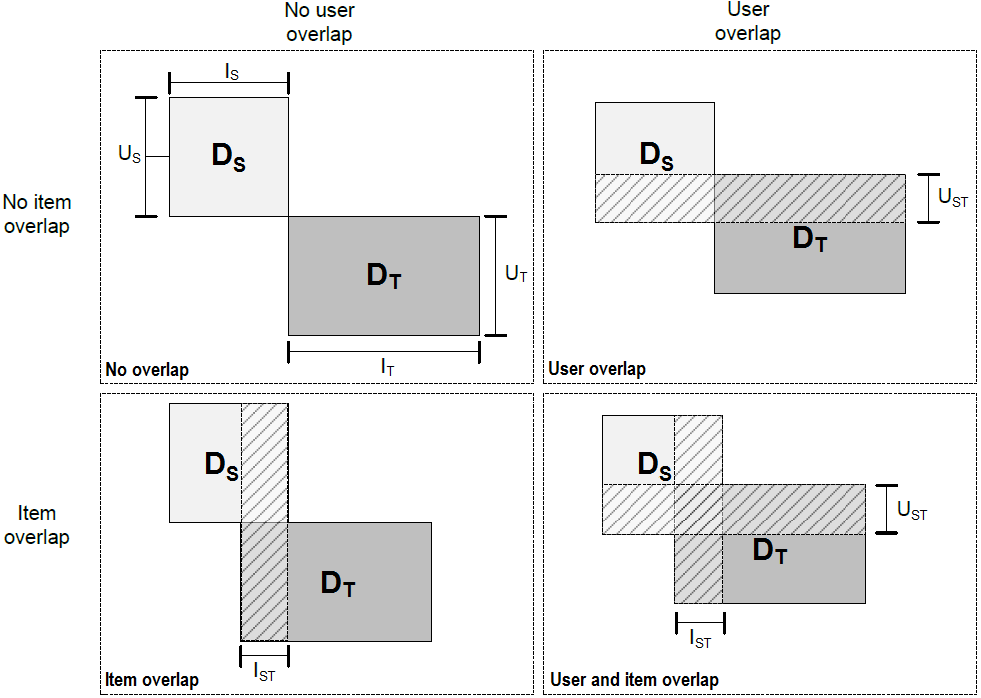
\includegraphics[width=\textwidth]{pictures/domains-overlap}
  \caption{Types of overlap of user and item sets between two domains. Source: https://doi.org/10.1007/978-1-4899-7637-6\_27}
\end{figure}


\subsection{Systems Categories}

Given the previous attributes, different cross-domain recommender system trends have been defined into a categorization by Loizou \cite{crossdomain-recsys-categorization}, which was later enhanced by Cremonesi \textit{et al} \cite{crossdomain-recsys-categorization} into four groups:
\begin{itemize}
\item As proposed by Lee \cite{10.1016/S0957-41740100034-3}, extract association rules from rating behavior in source domains, to be used in the target domain.
\item As proposed by Cao \textit{et al.} \cite{10.5555/3104322.3104344} and Zhang \textit{et al.} \cite{10.5555/3023549.3023635}, learn inter-domain similarity based on ratings and correlation matrices.
\item As proposed by Zhuang \textit{et al.} \cite{10.1109/TKDE.2009.205}, combine estimations of rating probability distributions in source domains, to be used in the target domain.
\item As proposed by Li \textit{et al.} \cite{10.5555/1661445.1661773, 10.1145/1553374.1553454} and Pan \textit{et al.} \cite{10.5555/2283696.2283784, 10.5555/2898607.2898644}, transfer knowledge from source domains to the target domain to reduce rating sparsity.
\end{itemize}
Furthermore, it is possible to make another type of distinction based on the approach of knowledge exploitation, into two macro-groups and sub-groups.
\begin{figure}[hbt!]
  \centering
  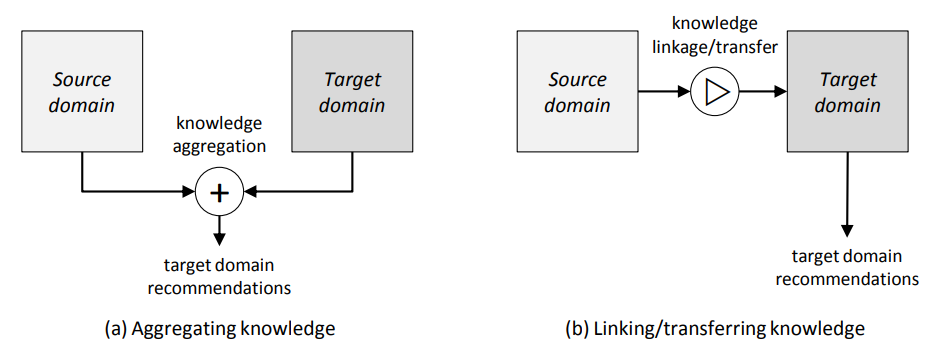
\includegraphics[width=\textwidth]{pictures/knowledge-exploitation}
  \caption{Types of knowledge exploitation in cross-domain recommender systems. Source: https://doi.org/10.1007/978-1-4899-7637-6\_27}
\end{figure}
\begin{itemize}
\item \textbf{Aggregating knowledge}
\begin{itemize}
\item \textbf{\textit{Merging user preferences}}: the aggregated knowledge consists of user preferences. Combining user profiles from multiple domains requires a single type of representation of user preferences.\\
This is the most used approach for cross domain recommendations. According to multiple sources \cite{10.1007/s11257-012-9131-2, 10.1007/978-3-540-88564-1_40, 10.1007/978-3-540-73078-1_44, 10.1145/1297231.1297238, 10.1007/s00354-008-0041-0}, by having user overlap between multiple domains and significant information about user preference in each domain, it is possible to extract a more complete user profile, to provide better recommendations with higher accuracy, by combining the user preferences in a single multi-domain profile. The aggregation of user preferences is able to provide knowledge about user tastes that cannot be extracted from a single domain.\\
According to others, aggregating user preferences is also beneficial to address the problem of cold-start \cite{10.1007/978-3-642-38844-6_25} and data sparsity \cite{10.1007/s11257-012-9128-x}.\\
While merging user preferences as ratings has proved the be the most efficient approach of building a multi-domain user profile, in real scenarios it is rarely possible to achieve a common represantion for ratings and to provide a sufficient user overlap, thus, more recent methods have focused on aggregating user tags. According to Szomszor \textit{et al.} \cite{10.1145/1379092.1379103, 10.1007/978-3-540-88564-1_40} it is possible to obtain higher quality recommendations by aggregating and correlating user social tags between domains. Such approach does not require user overlap.
\item \textbf{\textit{Mediating user modeling data}}: the aggregated knowledge consists of user models, such as similarities or neighbors.\\
This approach extends the previous one by aggregating information related to models of users and items. According to Berkovsky et al. \cite{10.1007/s11257-007-9042-9, 10.1007/11590323_22} this approach will enrich the user model and allow to provide higher quality recommendations in each aggregated domain.\\
For example, with the assumption of user overlap between domains, it is possible to merge the lists of user neighbors \cite{10.1145/1297231.1297238}. The same approach could be applied to item models.
\begin{figure}[hbt!]
  \centering
  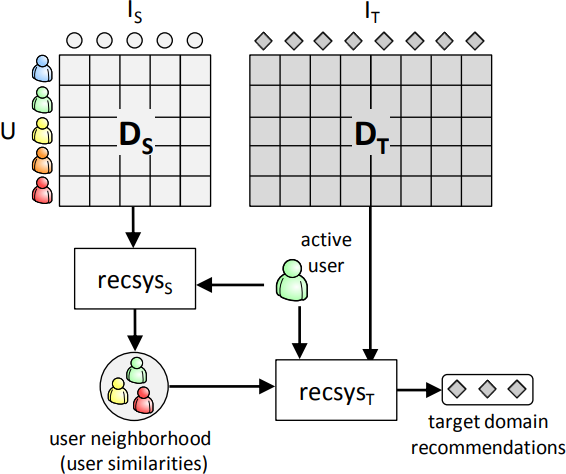
\includegraphics[width=0.8\textwidth]{pictures/mediating-user-modeling-data}
  \caption{Representation of the \textit{mediating-user-modeling-data} approach. Source: https://doi.org/10.1007/978-1-4899-7637-6\_27}
\end{figure}
\item \textbf{\textit{Combining recommendations}}: the aggregated knowledge is composed of single-domain recommendations.\\
In this approach, recommendations made in the source domains are used to enrich the recommendations in the target domain. Aggregating user recommendations requires both user and item overlap. While the recommendations in the single domains can be computed with different approaches, the challenge of this scenario is to compute weights for aggregation.
\begin{figure}[hbt!]
  \centering
  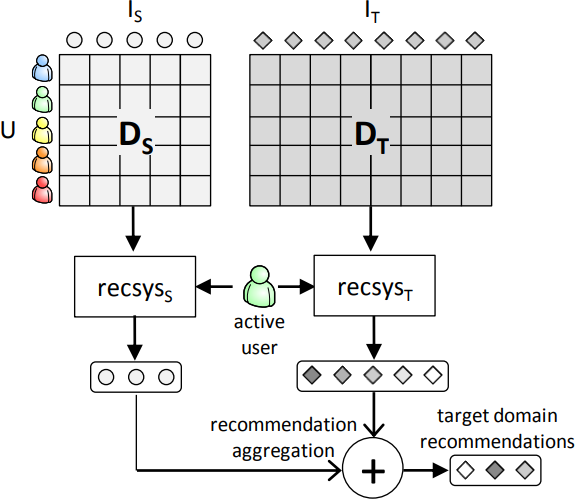
\includegraphics[width=0.8\textwidth]{pictures/combining-single-domain-recommendations}
  \caption{Representation of the \textit{combining-single-domain-recommendations} approach. Source: https://doi.org/10.1007/978-1-4899-7637-6\_27}
\end{figure}
\end{itemize}
\item \textbf{Linking and transferring knowledge}:
\begin{itemize}
\item \textbf{\textit{Linking domains}}: source and target domains are linked by common knowledge, such as item attributes.\\
This correspondences can either be directly identified between the single domains, or with the aid of an external domain. Despite no user or item overlap being needed for this approach, at least a partial feature overlap is required.\\
Chung \textit{et al.} \cite{10.1145/1282100.1282113} initially proposed an approach using item attributes directly to identify a bridge between domains, but since items are generally very heterogeneus, it may be difficult to find directly corresponding features. To address this problem, Loizou \cite{crossdomain-recsys-categorization} proposed to use Wikipedia as a universal vocabulary to express and relate user preferences across multiple domains.\\
The known problem of both approaches is building said knowledge repositories. Cremonesi \textit{et al.} \cite{10.1007/978-1-4899-7637-6_27} observed that the majority of approaches with the goal of linking domains does not require user or item overlap, but only feature overlap between domains. It was also observed that no particular approach outperforms the others in a general scenario.
\begin{figure}[hbt!]
  \centering
  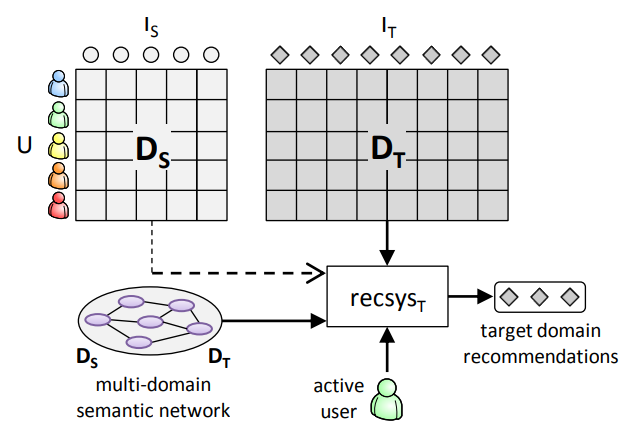
\includegraphics[width=0.8\textwidth]{pictures/linking-domains}
  \caption{Representation of the \textit{linking domains} approach. Source: https://doi.org/10.1007/978-1-4899-7637-6\_27}
\end{figure}
\item \textbf{\textit{Sharing latent features}}: source and target domains are linked by common latent features, such as extracted item features.\\
This approach is similar to the previous one, although it assumes that using denser representations of user preferences or item attributes, which are usually both very sparse sets, leads to more accurate matches \cite{10.5555/2283696.2283784, 10.5555/2898607.2898644}. These new representations are obtained with various factorization algorithms. Like for the previous approach, at least a feature overlap is strictly needed.
\begin{figure}[hbt!]
  \centering
  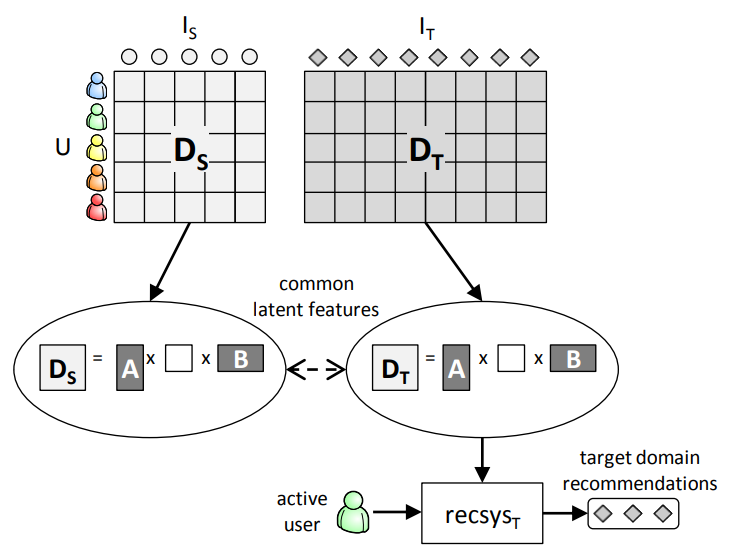
\includegraphics[width=0.8\textwidth]{pictures/sharing-latent-features}
  \caption{Representation of the \textit{sharing latent features} approach. Source: https://doi.org/10.1007/978-1-4899-7637-6\_27}
\end{figure}
\item \textbf{\textit{Transferring rating patterns}}: the rating pattern extracted from one or more source domains is transferred and applied in the target domain.\\
The base assumption of this approach is that similar domains share the population used to sample user preferences, even if there is no user or item overlap between them. For this reason it may be possible to find a correlation between domains of the preferences of groups of users for groups of items. This correlation is called \textit{rating pattern}. Thus, the rating pattern is the only information transferred from source domains to the target domain.\\
The first approach to transfer the rating pattern between domains was proposed by Li \textit{et al.} \cite{10.5555/1661445.1661773} and named \textit{codebook transfer}. Since then, several variants of codebook transfer have surfaced, all based on the same assumptions.\\
Being the focus of this thesis for evaluation purposes, the details of the codebook transfer theoretical model and its extensions are addressed in \autoref{theoretical-model}.
\begin{figure}[hbt!]
  \centering
  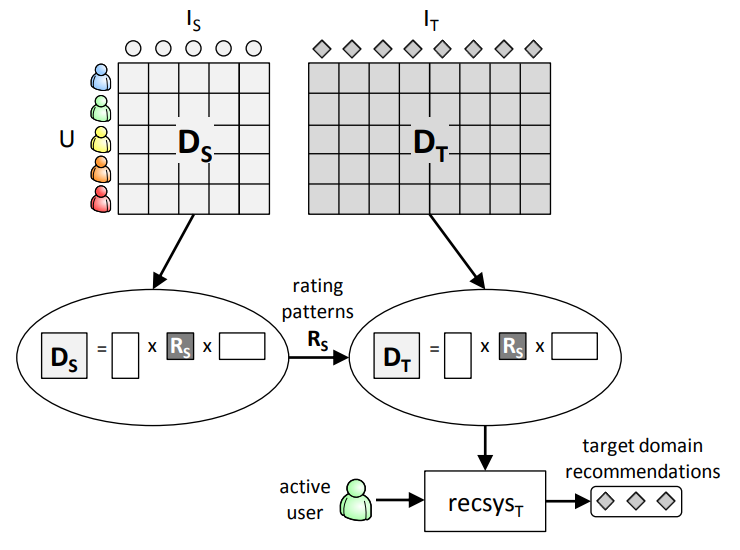
\includegraphics[width=0.8\textwidth]{pictures/transferring-rating-patterns}
  \caption{Representation of the \textit{transferring rating patterns} approach. Source: https://doi.org/10.1007/978-1-4899-7637-6\_27}
\end{figure}
\end{itemize}
\end{itemize}
Since in this thesis we evaluate the codebook transfer technique, we will focus on transferring knowledge and, in particular, on transferring rating patterns.
\chapter{Theoretical Model}
\label{ch:theoretical-model}

In this chapter we will cover the structure of the codebook transfer model, as provided by Li \textit{et al.} \cite{10.5555/1661445.1661773}, and explore the variant proposed by Zang \textit{et al.}, called LKT-FM \cite{10.1007/978-3-319-71246-8_39}.


\section{Codebook Transfer (CBT)}

CBT is a cross-domain recommender system aiming to transfer the rating pattern from a source domain to a target domain, to improve data quantity and provide better recommendations in the target domain. According to Li \textit{et al.} \cite{10.5555/1661445.1661773} CBT "can transfer useful knowledge from the auxiliary rating matrix in some other domains to remedy the sparsity of the rating matrix in a target domain".\\
Due to the nature of the model, we can distinguish three phases: codebook construction, codebook transfer and top-k recommendation.


\subsection{Input Data}

Input data provided to the CBT model consists in two user-rating matrices. We call $URM_S$ the user-rating matrix of the source domain and $URM_T$ the user-rating matrix of the target domain.\\
While no user or item overlap is not required, CBT has only requirement for input data: the sparsity of the source dataset should be low enough to allow a meaningful amount of knowledge to be transferred. In \cite{10.5555/1661445.1661773} Li \textit{et al.} did not provide a functional sparsity percentage. In their experiment, the source dataset had a sparsity lower than 50\%.


\subsection{Codebook Construction}

Codebook construction exploits the assumption that, in CF, users with similar tastes or items with similar attributes behave similarly. For this reason, it is possible to compute user and item clusters to obtain a much more compact user-rating matrix of the source domain, which represents the groups behavior. The obtained compact user-rating matrix is called \textit{codebook}.\\
Li \textit{et al.} provided the following definition for \textit{codebook}:\\
\begin{quotation}
"Codebook is a $k \times l$ matrix which compresses the cluster-level user-item rating patterns of $k$ user clusters and $l$ item clusters in the original rating matrix."
\end{quotation}
Once the codebook has been computed, an approximation of the original user-rating matrix can be retrieved.\par
The codebook construction has to be performed by clustering users and items simultaneously. The authors adopted ONMTF \cite{10.1145/1150402.1150420} as the clustering algorithm. Thus, given a source user-rating matrix $X_S$ with shape $n \times m$ and a target codebook size $k \times l$, the optimization problem is the following:
\begin{equation}
\min_{U_S \in \mathbb{R}^{n \times k}_+, V_S \in \mathbb{R}^{m \times l}_+, S \in \mathbb{R}^{k \times l}_+} \norm{X_S - U_S S V_S^T}_F^2, \quad \text{s.t.} \quad U_S^T U_S = I, V_S^T V_S = I
\end{equation}
Where $U_S$ is the matrix of user clusters indicators and $V_S$ is the matrix of item clusters indicators.\\
$U_S$, $V_S$ and $S$ can be initialized randomly or with K-Means.\\
Since it is sufficient to obtain a cluster hard membership indicator for each user and item, $U_S$ and $V_S$ are binarized to have only the non-negative entry in each row set to 1 and the others set to 0.\\
Once $U_S$ and $V_S$ are computed, the codebook $B$ is computed as follows:
\begin{equation}
\label{eq:codebook-construction}
B = \frac{U_S^T X_S V_S}{U_S^T 11^T V_S}
\end{equation}
The complete algorithm for codebook construction is the following:
\vskip 0.7cm
\begin{algorithm}[H]
\SetKwInOut{Input}{Input}
\SetKwInOut{Output}{Output}
\Input{The source domain user-rating matrix $X_S \in \mathbb{R}^{n \times m}$;\\
The amount of user and item clusters $k$ and $l$.}
\Output{A codebook $B \in \mathbb{R}^{k \times l}$ learned from $X_S$.}
Initialize $U_S^{(0)}$, $V_S^{(0)}$, $S^{(0)}$ randomly or with K-Means\;
\For{$t \gets 1$ \KwTo $max\_iteration$}
{
  Update $U_S$, $V_S$ and $S$ using the following equations:\\
  $V_S^{(t)} \gets V_S^{(t - 1)} \odot \sqrt{\frac{X_S^T U_S^{(t - 1)} S^{(t - 1)}}{V_S^{(t - 1)} [V_S^{(t - 1)}]^T X_S^T U_S^{(t - 1)} S^{(t - 1)}}}$\;
  $U_S^{(t)} \gets U_S^{(t - 1)} \odot \sqrt{\frac{X_S V_S^{(t)} [S^{(t - 1)}]^T}{U_S^{(t - 1)} [U_S^{(t - 1)}]^T X_S V_S^{(t)} [S^{(t - 1)}]^T}}$\;
  $S^{(t)} \gets S^{(t - 1)} \odot \sqrt{\frac{[U_S^{(t)}]^T X_S V_S^{(t)}}{[U_S^{(t)}]^T U_S^{(t)} S^{(t - 1)} [V_S^{(t)}]^T V_S^{(t)}}}$\;
}
Allocate spaces for $U_S$ and $V_S$\;
\For{$i \gets 1$ \KwTo $n$}
{
  $\hat{j} = argmax_{j \in (1,...,k)}(U_{ij})$\;
  $[U_S]_{i\hat{j}} \gets 1$\;
  \For{$j \in (1,...,k)/\hat{j}$}
  {
    $[U_S]_{ij} \gets 0$\;
  }
}
\For{$i \gets 1$ \KwTo $m$}
{
  $\hat{j} = argmax_{j \in (1,...,l)}(V_{ij})$\;
  $[V_S]_{i\hat{j}} \gets 1$\;
  \For{$j \in (1,...,l)/\hat{j}$}
  {
    $[V_S]_{ij} \gets 0$\;
  }
}
Compute $B$ using \autoref{eq:codebook-construction}:\\
$B = \frac{U_S^T X_S V_S}{U_S^T 11^T V_S}$;
\caption{The algorithm for codebook construction}
\end{algorithm}
\vskip 0.7cm
According to Li \textit{et al.}, too many clusters can comprise redundant information, while too few cluster could be insufficient to encode the users and items information, missing important knowledge. An optimal codebook size should be expressive enough and suitable for computation.
\begin{figure}[hbt]
  \centering
  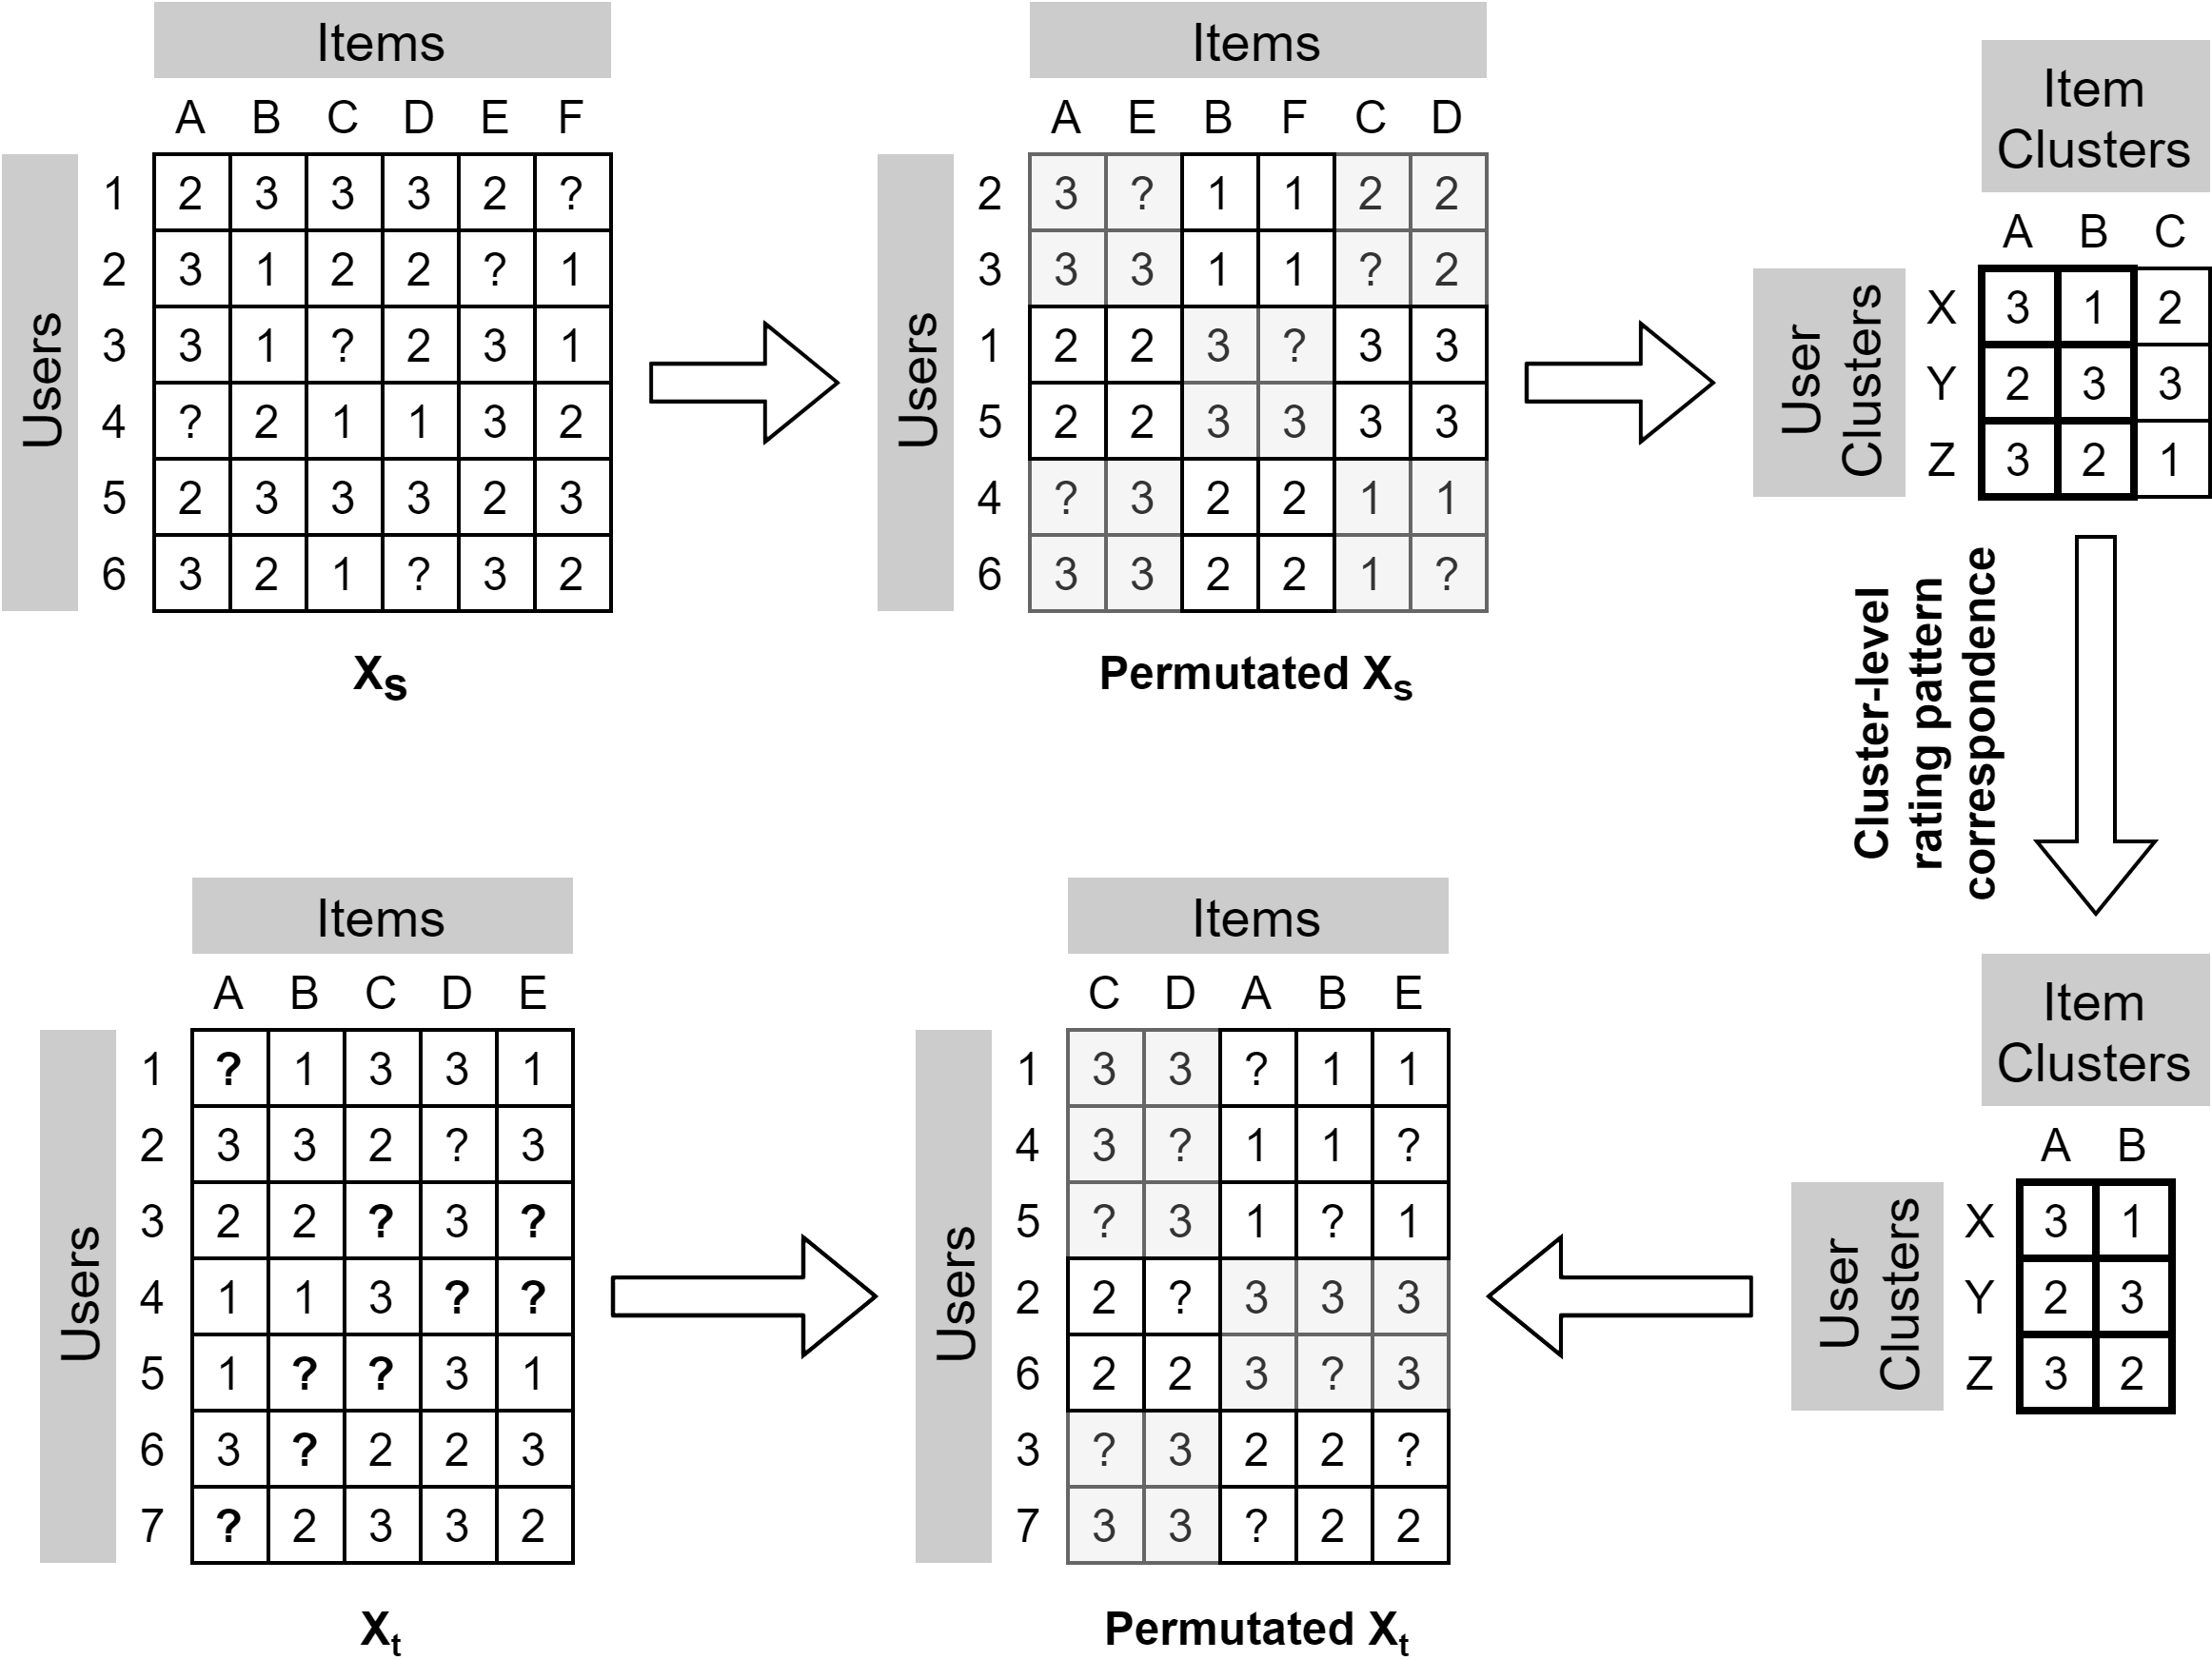
\includegraphics[width=0.8\textwidth]{pictures/codebook-construction}
  \caption
  [Example of codebook construction. Source: https://dl.acm.org/doi/10.5555/1661445.1661773]
  {\protect\raggedright Example of codebook construction. Source: https://dl.acm.org/doi/10.5555/1661445.1661773}
\end{figure}


\subsection{Codebook Transfer}
\label{sc:codebook-transfer}

\begin{figure}[hbt]
  \centering
  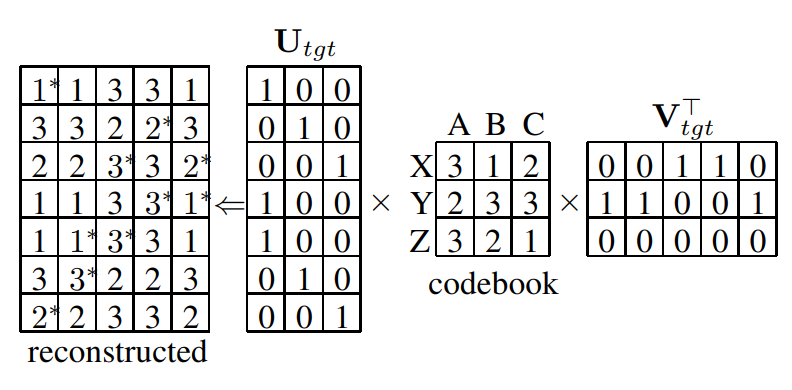
\includegraphics[width=0.8\textwidth]{pictures/codebook-transfer}
  \caption
  [Example of codebook transfer. Source: https://dl.acm.org/doi/10.5555/1661445.1661773]
  {\protect\raggedright Example of codebook transfer. Source: https://dl.acm.org/doi/10.5555/1661445.1661773}
\end{figure}
Having constructed the codebook $B$, the model applies it to the target domain. To do this, it assumes that there is correspondence of user and item clusters between the two domains. Transferring the rating pattern consists in the inverse operation to codebook construction. The codebook is expanded to reconstruct an approximation of the target user-rating matrix $X_T$.\\
The duplication of a row or column of the codebook implies that there is a set of users or items in the target domain that behaves like the cluster represented by the row or column.\\
Once an approximation of $X_T$ has been obtained, it is suitable to exclude the already observed ratings in order to predict only the missing entries.\\
The minimization problem for codebook transfer is defined as follows:
\begin{equation}
\min_{U_T \in \{0,1\}^{p \times k}, V_T \in \{0,1\}^{q \times l}} \norm{[X_T - U_T B V_T^T] \odot W}_F^2, \quad \text{s.t.} \quad U_T 1 = 1, V_T 1 = 1
\end{equation}
where $U_T$ and $V_T$ are the matrices of cluster membership, respectively for users and items, such that:
\begin{equation}
  [U_T]_{ij} =
  \begin{cases}
    0, & \text{if user}\ [X_T]_{i}\ \text{belongs to cluster}\ j\\
    1, & \text{otherwise}
  \end{cases}
  , \quad \text{s.t.} \quad i \in \{1,p\}, j \in \{1,k\}
\end{equation}
\begin{equation}
  [V_T]_{ij} =
  \begin{cases}
    0, & \text{if item}\ [X_T]_{i}\ \text{belongs to cluster}\ j\\
    1, & \text{otherwise}
  \end{cases}
  , \quad \text{s.t.} \quad i \in \{1,q\}, j \in \{1,l\}
\end{equation}
and $W$ is the masking matrix with shape $p \times q$ such that:
\begin{equation}
  W_{ij} =
  \begin{cases}
    0, & \text{if}\ [X_T]_{ij}\ \text{is not rated}\\
    1, & \text{otherwise}
  \end{cases}
  , \quad \text{s.t.} \quad i \in \{1,p\}, j \in \{1,q\}
\end{equation}
Once $U_T$ and $V_T$ have been obtained, it is possible to expand the codebook and fill the target user-rating matrix as follows:
\begin{equation}
\label{eq:codebook-transfer-fill}
\bar{X_T} = W \odot X_T + [1 - W] \odot [U_T B V_T^T]
\end{equation}
The complete algorithm for codebook transfer is the following:
\vskip 0.7cm
\begin{algorithm}[H]
\SetKwInOut{Input}{Input}
\SetKwInOut{Output}{Output}
\Input{The codebook $B \in \mathbb{R}^{k \times l}$ learned from $X_S$;\\
The target domain user-rating matrix $X_T \in \mathbb{R}^{p \times q}$;\\
The masking matrix $W \in \{0,1\}^{p \times q}$.}
\Output{The filled target domain user-rating matrix $\bar{X_T}$.}
Allocate spaces for $U_S$ and $V_S$\;
\For{$i \gets 1$ \KwTo $m$}
{
  $\hat{j} =\ \text{random from}\ \{1,...,l\}$\;
  $[V_T^{(0)}]_{i\hat{j}} \gets 1$\;
  \For{$j \in (1,...,l)/\hat{j}$}
  {
    $[V_T^{(0)}]_{ij} \gets 0$\;
  }
}
\For{$t \gets 1$ \KwTo $max\_iteration$}
{
  \For{$i \gets 1$ \KwTo $p$}
  {
    $\hat{j} = argmin_j \norm{[X_T]_{i*} - [B [V_T^{(t - 1)}]^T]_{j*}}_{W_{i*}}^2$\;
    $[U_T^{(t)}]_{i\hat{j}} \gets 1$\;
    \For{$j \in (1,...,k)/\hat{j}$}
    {
      $[U_T^{(t)}]_{ij} \gets 0$\;
    }
  }
  \For{$i \gets 1$ \KwTo $q$}
  {
    $\hat{j} = argmin_j \norm{[X_T]_{*i} - {[U_T^{(t - 1)} B]}_{*j}}_{W_{*i}}^2$\;
    $[V_T^{(t)}]_{i\hat{j}} \gets 1$\;
    \For{$j \in (1,...,l)/\hat{j}$}
    {
      $[V_T^{(t)}]_{ij} \gets 0$\;
    }
  }
}
Compute $X_T$ using \autoref{eq:codebook-transfer-fill}:
$\bar{X_T} = W \odot X_T + [1 - W] \odot [U_T B V_T^T]$\;
\caption{The algorithm for codebook transfer}
\label{al:codebook-transfer}
\end{algorithm}
\vskip 0.7cm
The following passages prove that the codebook transfer algorithm monotically reduces the loss function. In particular it needs to be proved that the following inequalities always hold:
\begin{equation}
\label{eq:codebook-transfer-monotone-1}
\begin{split}
& \norm{[X_T - U_T^{(t - 1)} B [V_T^{(t - 1)}]^T] \odot W}_F^2 \\
\geq & \norm{[X_T - U_T^{(t)} B [V_T^{(t - 1)}]^T] \odot W}_F^2
\end{split}
\end{equation}
\begin{equation}
\label{eq:codebook-transfer-monotone-2}
\begin{split}
& \norm{[X_T - U_T^{(t)} B [V_T^{(t - 1)}]^T] \odot W}_F^2 \\
\geq & \norm{[X_T - U_T^{(t)} B [V_T^{(t)}]^T] \odot W}_F^2
\end{split}
\end{equation}
First, the authors prove \autoref{eq:codebook-transfer-monotone-1}, where $U_T$ is updated and $V_T$ is fixed. It is possible to state that:
\begin{equation}
\label{eq:codebook-transfer-monotone-3}
\begin{split}
& \norm{[X_T - U_T^{(t - 1)} B [V_T^{(t - 1)}]^T] \odot W}_F^2 \\
= & \sum_{i = 1}^{n} \sum_{j = 1}^{k} [U_T^{(t - 1)}]_{ij} \norm{[X_T]_{i*} - [B [V_T^{(t - 1)}]^T]_{j*}}_{W_{i*}}^2 \\
= & \sum_{i = 1}^{n} \norm{[X_T]_{i*} - [B [V_T^{(t - 1)}]^T]_{\delta([U_T^{(t - 1)}]_{i*})}}_{W_{i*}}^2
\end{split}
\end{equation}
and, with the similar passages, that:
\begin{equation}
\begin{split}
& \norm{[X_T - U_T^{(t)} B [V_T^{(t - 1)}]^T] \odot W}_F^2 \\
= & \sum_{i = 1}^{n} \sum_{j = 1}^{k} [U_T^{(t)}]_{ij} \norm{[X_T]_{i*} - [B [V_T^{(t - 1)}]^T]_{j*}}_{W_{i*}}^2 \\
= & \sum_{i = 1}^{n} \norm{[X_T]_{i*} - [B [V_T^{(t - 1)}]^T]_{\delta([U_T^{(t)}]_{i*})}}_{W_{i*}}^2
\end{split}
\end{equation}
thus, it is possible to state that:
\begin{equation}
\begin{split}
& \sum_{i = 1}^{n} \norm{[X_T]_{i*} - [B [V_T^{(t - 1)}]^T]_{\delta([U_T^{(t - 1)}]_{i*})}}_{W_{i*}}^2 \\
\geq & \sum_{i = 1}^{n} \norm{[X_T]_{i*} - [B [V_T^{(t - 1)}]^T]_{\delta([U_T^{(t)}]_{i*})}}_{W_{i*}}^2
\end{split}
\end{equation}
where $[\cdot]_{i*}$ and $[\cdot]_{*i}$ denote the $i$-th row and column in a matrix, and
\begin{equation*}
\norm{X}_{W_{i*}}^2 = X^T diag(W_{i*}) X
\end{equation*}
is the $l_2$-norm.\\
The function $\delta(\cdot)$ returns the index of the largest value of a vector.\\
\autoref{eq:codebook-transfer-monotone-3} is obtained based on the fact that each user belongs to only one cluster. Thus it is possible to assume that $\exists! 1 \in [U_T^{(t - 1)}]_{i*}$ and the sum of $[U_T^{(t - 1)}]_{i*}$ weighted quadratic losses can be replaced by only one quadratic loss, indexed by the indicator function $\delta([U_T^{(t - 1)}]_{i*})$, which tells that the cluster to which the $i$-th user (i.e., $[X_T]_{i*}$) belongs at the $(t-1)$-th iterative round.\\
\autoref{eq:codebook-transfer-monotone-2} can be proved in the same way.


\subsection{Top-K Recommendations}

The third step of the codebook transfer model consists in using the filled target user-rating matrix to extract recommendations with a memory based collaborative filtering approach, such as nearest neighborhood.


\section{Low-Rank Knowledge Transfer via Factorization Machines (LKT-FM)}

LKT-FM is a codebook transfer variation proposed by Zang \textit{et al.} \cite{10.1007/978-3-319-71246-8_39} in 2017.\\
Similarly to the original codebook transfer model, it is comprised of three steps: codebook construction, codebook transfer, and recommendations extraction.


\subsection{Codebook Construction}

According to  Zang \textit{et al.}, constructing rating patterns through user-item co-clustering has potential issues when the source matrix is sparse. For this reason they propose a new construction method to alleviate this problem.\par
Given a source user-rating matrix $X_S$ with shape $m \times n$, a target codebook size $k \times l$, $X_S$ is processed with basic matrix factorization and factorized into two latent factor matrices: $U_S$, with shape $m \times d$, for users and $V_S$, with shape $n \times h$ for items, where $d$ and $h$ are the latent factors dimensions.\\
Then KMeans is applied to $U_S$ and $V_S$ to obtain cluster membership matrices $P_S$, with shape $m \times k$, for users and $Q_S$, with shape $n \times l$, for items.\\
Like in CBT, the codebook $B$ is computed with the following equation:
\begin{equation}
B = \frac{P_S^T X_S Q_S}{P_S^T 11^T Q_S}
\end{equation}
Further details about the codebook construction implementation are provided in \autoref{ch:applied-model}.


\subsection{Codebook Transfer}

Given the target user-rating matrix $X_T$, with shape $p \times q$, to map the user and item clusters, LKT-FM uses the same approach proposed by Li \textit{et al.} \cite{10.5555/1661445.1661773}. Thus \autoref{al:codebook-transfer} is used to obtain the cluster membership matrices $U_T$, with shape $p \times k$, for users and $V_T$, with shape $q \times l$ for items.\par
According to the authors, previous rating pattern transfer models do not work well in some conditions due to the integration method, which is usually that of expanding the codebook by duplicating its rows or columns. They named this method \textit{direct expansion}. Zang \textit{et al.} state that direct expansion may miss useful knowledge contained in the target user-rating matrix itself, thus the transferred knowledge could hurt the memory based collaborative filtering recommender performance. As a result, they propose a new integration method based on factorization machines.\par
In LKT-FM, instead of expanding $B$ by duplicating its rows and columns, like in the original codebook transfer model, the target user-rating matrix is filled by using factorization machines.\\
Given the target domain $D_T$ and the user and item sets $U_T$ and $I_T$, the rating prediction problem for $D_T$ is modeled by a target function $f: U_T \times I_T \rightarrow \mathbb{R}$. Using factorization machines, each user-item interaction $(u,i) \in U_T \times I_T$ in $X_T$ is represented by a feature vector $x_{ui} \in \mathbb{R}^k$, where $k = \abs{U_T} + \abs{I_T}$, containing binary values that represent which user rated which item. For each entry $(u,i) \in X_T$, the corresponding feature vector $x$ can be represented as:
\begin{equation}
x_{ui} = (\underbrace{0,...,1,...,0}_{\abs{U_T}},\underbrace{0,...,1,...,0}_{\abs{I_T}})
\end{equation}
It is then possible to expand $x_{ui}$ with other features, such as cluster membership from matrices $U_T$ and $V_T$ and the codebook rating, to obtain the following representation:
\begin{equation}
x_{ui} = (\underbrace{0,...,1,...,0}_{\abs{U_T}},\underbrace{0,...,1,...,0}_{\abs{I_T}},\underbrace{0,...,1,...,0}_{k},\underbrace{0,...,1,...,0}_{l},B_{C_uC_i})
\end{equation}
where $k$ and $l$ are the amount of user and item clusters and $B_{C_uC_i}$ is the codebook rating of users of cluster $C_u$ to items of cluster $C_i$. In the added part, the $k$ binary indicator represent which cluster the user belongs to and the $l$ binary indicator represents which cluster the item belongs to.\\
The feature vector $x_{ui}$ is then used as input for a factorization machine. The output $y$ represents the predicted rating of user $u$ to item $i$.
\begin{figure}[hbt]
  \centering
  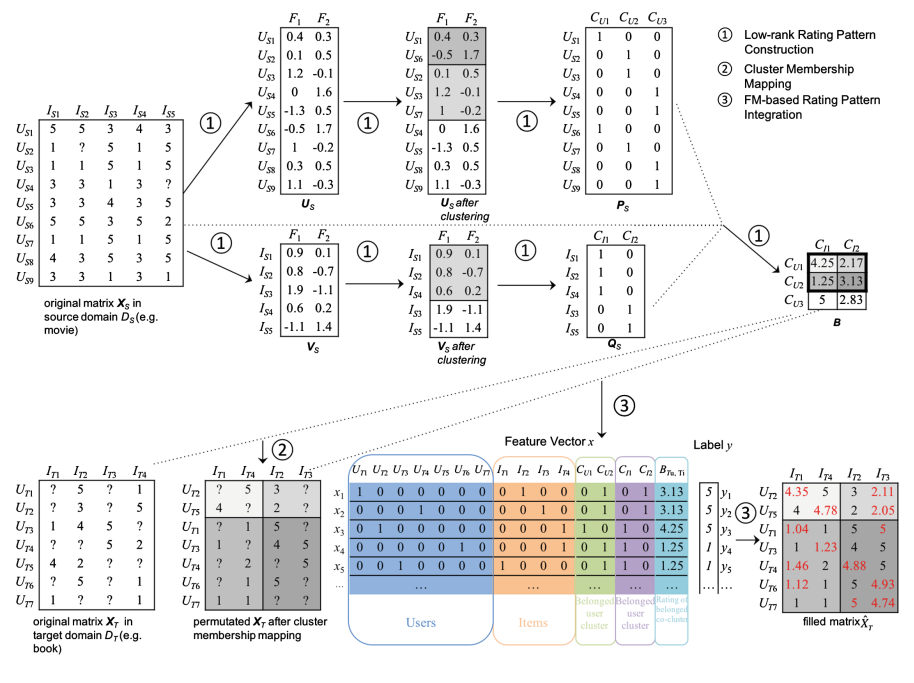
\includegraphics[width=\textwidth]{pictures/lkt-fm}
  \caption
  [Representation of the LKT-FM model. Source: https://doi.org/10.1007/978-3-319-71246-8\_39]
  {\protect\raggedright Representation of the LKT-FM model. Source: https://doi.org/10.1007/978-3-319-71246-8\_39}
\end{figure}
\chapter{Applied Model}
\label{ch:applied-model}

In this chapter we will cover the model implementations of CBT and LKT-FM. Both models are implemented using the Python programming language version 3.6 and multiple libraries, such as \textit{Numpy} \cite{10.1109/MCSE.2011.37} and \textit{Scipy} \cite{scipy} for matrix computation and \textit{Scikit-learn} \cite{10.5555/1953048.2078195} to compute KMeans. The experiments are built upon the RecSys@Polimi framework by Maurizio Ferrari Dacrema \cite{recsys-polimi-framework}, which offers dataset readers, baseline recommender systems, similarity computation and evaluation metrics.



\section{Hyperparameter Tuning}

To perform experiments, hyperparameters for each model are optimized using a wrapper of Scikit-optimize \cite{10.5281/zenodo.1170575} for bayesian optimization.\\
Bayesian optimization \cite{bayesian-optimization} is a method to optimize black-box functions that take long time to evaluate by building a surrogate for the objective and quantifying the uncertainty in that surrogate using a bayesian machine learning technique called \textit{Gaussian process regression}. It then uses an acquisition function defined from this surrogate to decide where to sample in the provided hyperparameter ranges.\\
The wrapper accepts as input a set of hyperparameter ranges, an amount of cases, which is the number of runs of training and evaluation to perform, an amount of random starts, which is the numbers of times the optimization process will initialize the hyperparameters randomly within the provided range, and a target evaluation metric, used to perform comparison between runs.\\
Each training and evaluation run during hyperparameter tuning is performed using a training dataset and a validation dataset, which has the same properties as the final test dataset while they are disjoint.\\
Further details about the hyperparameters and other tuning variables are covered in the single experiments in \autoref{ch:experiments}.



\section{CBT}


\subsection{Codebook Construction}

Since ONMTF does not monotically decrease the function, we opted for and early stopping approach to ensure a suitable amount of iterations.\\
The code for ONMFT is as follows:
\begin{minted}[breaklines]{python}
import numpy as np
from numpy.linalg import multi_dot
from sklearn.cluster import KMeans

def initialize(self, X_s, k, l):

    # Source user-rating matrix
    self.X_s = X_s
    self.m, self.n = X.shape
    # Amount of codebook user clusters
    self.k = k
    # Amount of codebook item clusters
    self.l = l
    # ONMTF factorization matrices
    self.F = None
    self.G = None
    self.S = None
    
    # Initialize the factorization matrices
    _initialize_clustering()

def update():
    _update_G()
    _update_F()
    _update_S()
    return _loss()

def _initialize_clustering():
    """
    Initialize F, G, and S latent matrices according to Ding et al. 2006:
    1. G is obtained via k means clustering of columns of X_s. G = G + 0.2
    2. F is obtained via k means clustering of rows of X_s. F = F + 0.2
    3. S is obtained via S = F.T @ X_s @ G
    """
    self.G = _cluster(self.X_s.T, self.l)
    self.G += 0.2
    self.F = _cluster(self.X_s, self.k)
    self.F += 0.2
    self.S = multi_dot([self.F.T, self.X_s, self.G])
    
def _cluster(X, k):
    kmeans = KMeans(n_clusters=k, random_state=0).fit(X)
    labels = set(kmeans.labels_)
    labeled_features = kmeans.labels_
    return np.array([np.multiply([i == k for i in labeled_features], 1) for k in labels]).T.astype(np.float64)

def _update_G():
    enum = multi_dot([self.X_s.T, self.F, self.S])
    denom = multi_dot([self.G, self.G.T, self.X_s.T, self.F, self.S])
    self.G *= np.nan_to_num(np.sqrt(enum / denom))

def _update_F():
    enum = multi_dot([self.X_s, self.G, self.S.T])
    denom = multi_dot([self.F, self.F.T, self.X_s, self.G, self.S.T])
    self.F *= np.nan_to_num(np.sqrt(enum / denom))

def _update_S():
    enum = multi_dot([self.F.T, self.X_s, self.G])
    denom = multi_dot([self.F.T, self.F, self.S, self.G.T, self.G])
    self.S *= np.nan_to_num(np.sqrt(enum / denom))

def _loss():
    FSGt = multi_dot([self.F, self.S, self.G.T])
    loss = np.linalg.norm(self.X_s - FSGt)
    return loss
\end{minted}
where the \textit{update} function is called by the framework with an early stopping approach.\\
The matrix binarization and codebook construction is then performed as follows:
\begin{minted}[breaklines]{python}
def codebook_construction(X_s, F, G):

    F = _binarize_matrix(F)
    G = _binarize_matrix(G)
    
    sum_vector = np.ones(X.shape)
    enum = multi_dot([F.T, X_s, G])
    denom = multi_dot([F.T, sum_vector, G])
    
    B = np.nan_to_num(enum / denom)
    return B
    
def _binarize_matrix(X):
    """
    Binarize input matrix with 0 and 1
    """
    for i in range(X.shape[0]):
        # Find largest score in the row
        max_score = sorted(list(X[i, :])).pop()
        # Replace all other scores into 0
        X[i, :] = np.where(X[i, :] == max_score, X[i, :], 0)
        # Replace largest score with 1
        X[i, :] = np.where(X[i, :] == 0, X[i, :], 1)
    return X_copy
\end{minted}


\subsection{Codebook Transfer}

The codebook transfer technique provided in \autoref{sc:codebook-transfer} monotically decreases the loss function. Thus it is enough to stop the algorithm on the iteration in which the loss function returns a value equal to the one of the previous iteration.\\
Since the algorithm always converges to a local minimum, it is possible to run it several times to further minimize the loss function in alternative local minima.\\
The code for codebook transfer is as follows:
\begin{minted}[breaklines]{python}
import numpy as np
from numpy.linalg import multi_dot

def initialize(X_t, B, transfer_attempts, maximum_fill_iterations):

    # Target user-rating matrix  to be filled
    self.X_t = X_t
    self.p, self.q = X_t.shape
    # Codebook
    self.B = B
    self.k, self.l = B.shape
    # Amount of searches for different local minima to perform
    self.transfer_attempts = transfer_attempts
    # Maximum iterations to perform before the attempt is forced to stop
    self.maximum_fill_iterations = maximum_fill_iterations
    # Masking matrix
    self.W = None
    self.W_flipped = None
    # Factorization matrices
    self.U = None
    self.V = None
    self.U_best = None
    self.V_best = None
    # Best loss until now
    self.loss_best = np.inf
    
    # Initialize the masking matrix
    _generate_W()
    
    # Search local minima
    for attempt in range(self.transfer_attempts):
    
        _initialize_U()
        _initialize_V()
        iteration_loss_best = np.inf
        
        for i in range(self.maximum_fill_iterations):
            _update_U()
            _update_V()
            # Remove the filled values from the generated target matrix and compare it to the original one
            loss = np.linalg.norm((self.X_t - multi_dot([self.U, self.B, self.V.T])) * self.W)
            # The loss function is monotone, so stop if we have reached the local minimum
            if loss == iteration_loss_best:
                break
            iteration_loss_best = loss

        # Generate multiple local minima and keep the best one
        if iteration_loss_best < self.loss_best:
            self.loss_best = iteration_loss_best
            self.U_best = self.U
            self.V_best = self.V

def fill_matrix():
    prediction = self.W_flipped * multi_dot([self.U_best, self.B, self.V_best.T])
    X_t_filled = self.W * self.URM_target_train + prediction
    return X_t_filled

def _generate_W():
    self.W = np.zeros((self.p, self.q))
    self.W = np.divide(self.URM_target_train, self.URM_target_train)
    self.W = np.nan_to_num(self.W)
    self.W_flipped = 1 - self.W

def _initialize_U():
    self.U = np.zeros((self.p, self.k))

def _initialize_V():
    self.V = np.zeros((self.q, self.l))
    for i in range(self.q):
        j = np.random.randint(self.l)
        self.V[i, j] = 1.0

def _update_U():
    BV_t = np.dot(self.B, self.V.T)
    for i in range(self.p):
        loss = np.ndarray(self.k)
        for j in range(self.k):
            loss[j] = np.linalg.norm((self.X_t[i, :] - BV_t[j, :]) * self.W[i, :])
        j = np.argmin(loss)
        self.U[i, :] = 0.0
        self.U[i, j] = 1.0

def _update_V():
    UB = np.dot(self.U, self.B)
    for i in range(self.q):
        loss = np.ndarray(self.l)
        for j in range(self.l):
            loss[j] = np.linalg.norm((self.X_t[:, i] - UB[:, j]) * self.W[:, i])
        j = np.argmin(loss)
        self.V[i, :] = 0.0
        self.V[i, j] = 1.0
\end{minted}


\section{LKT-FM}


\subsection{Codebook Construction}


\subsection{Codebook Transfer}
\chapter{System Architecture}
\chapter{Results}
\chapter{Conclusion}
\label{ch:conclusion}

In the previous chapters we analysed the state of the art of pattern transfer recommender systems. Moreover we focused on its variant without overlap, currently known as codebook transfer. Codebook transfer, given a meaningful source domain, should be able to alleviate the data quantity and cold start problems of a target domain by filling the data gaps with knowledge extracted from the rating pattern of groups of users.\par
In our ranking experiments we compared the original codebook transfer method and LKT-FM, an evolution of it, with multiple baselines, with various combinations of well known source and target datasets. Each experiment includes comparisons with random, top popular items and $k$-nearest neighbors without knowledge transfer recommender systems. The results provide evidence that the performance of codebook transfer is inferior to the one of classic recommender systems, such as $k$-nearest neighbors without knowledge transfer and, in some cases, top popularity items recommendation.\\
Furthermore, by expanding on the previous experiments by Cremonesi and Quadrana on rating prediction, it is possible to say that codebook transfer can apparently improve error metrics without transferring knowledge, due to its nature being very similar to that of SVD matrix factorization in the codebook transfer phase.\\
For this same reason, it is not suitable for the ranking task as, indeed, it mostly fills the target user-rating matrix with noise. To prove this, we applied various transformations to the source domain, including rating removal and random generation, and obtained very similar results to the ones obtained with the original source domain.\\
Results including LKT-FM also underline that the derived approach, that employs an alternative codebook expansion method using factorization machines, is outperformed by almost every baseline, having similar performance to the random recommender system.\par
To summarize, in this thesis we aim to expand on the outcome of previous evaluations with theoretical and empirical evidence that the original codebook transfer method and its derived approaches are not capable of providing solid knowledge transfer between non-overlapping domains.\\
Future research may be focused on providing alternative methods to extract meaningful knowledge from source domains.

\cleardoublepage
% ---- Bibliography ----
\addcontentsline{toc}{chapter}{Bibliografia}
\bibliographystyle{plain}
\bibliography{bibl_tesi}
%\nocite{*}

\appendix

\pagestyle{fancy} 
\fancyfoot{}                                               
\renewcommand{\chaptermark}[1]{\markboth{\appendixname\ \thechapter.\ #1}{}} 
\renewcommand{\sectionmark}[1]{\markright{\thesection.\ #1}}         
\fancyhead[LE,RO]{\bfseries\thepage}    
                                        
\fancyhead[RE]{\bfseries\leftmark}    
\fancyhead[LO]{\bfseries\rightmark}     
\renewcommand{\headrulewidth}{0.3pt} 

%\include{appendiceA}
%\include{appendiceB}
%\include{appendiceC}
%\include{appendiceD}
%\include{appendiceE}
%\include{appendiceF}

\end{document}